\documentclass{article}\usepackage[]{graphicx}\usepackage[]{color}
%% maxwidth is the original width if it is less than linewidth
%% otherwise use linewidth (to make sure the graphics do not exceed the margin)
\makeatletter
\def\maxwidth{ %
  \ifdim\Gin@nat@width>\linewidth
    \linewidth
  \else
    \Gin@nat@width
  \fi
}
\makeatother

\definecolor{fgcolor}{rgb}{0.345, 0.345, 0.345}
\newcommand{\hlnum}[1]{\textcolor[rgb]{0.686,0.059,0.569}{#1}}%
\newcommand{\hlstr}[1]{\textcolor[rgb]{0.192,0.494,0.8}{#1}}%
\newcommand{\hlcom}[1]{\textcolor[rgb]{0.678,0.584,0.686}{\textit{#1}}}%
\newcommand{\hlopt}[1]{\textcolor[rgb]{0,0,0}{#1}}%
\newcommand{\hlstd}[1]{\textcolor[rgb]{0.345,0.345,0.345}{#1}}%
\newcommand{\hlkwa}[1]{\textcolor[rgb]{0.161,0.373,0.58}{\textbf{#1}}}%
\newcommand{\hlkwb}[1]{\textcolor[rgb]{0.69,0.353,0.396}{#1}}%
\newcommand{\hlkwc}[1]{\textcolor[rgb]{0.333,0.667,0.333}{#1}}%
\newcommand{\hlkwd}[1]{\textcolor[rgb]{0.737,0.353,0.396}{\textbf{#1}}}%

\usepackage{framed}
\makeatletter
\newenvironment{kframe}{%
 \def\at@end@of@kframe{}%
 \ifinner\ifhmode%
  \def\at@end@of@kframe{\end{minipage}}%
  \begin{minipage}{\columnwidth}%
 \fi\fi%
 \def\FrameCommand##1{\hskip\@totalleftmargin \hskip-\fboxsep
 \colorbox{shadecolor}{##1}\hskip-\fboxsep
     % There is no \\@totalrightmargin, so:
     \hskip-\linewidth \hskip-\@totalleftmargin \hskip\columnwidth}%
 \MakeFramed {\advance\hsize-\width
   \@totalleftmargin\z@ \linewidth\hsize
   \@setminipage}}%
 {\par\unskip\endMakeFramed%
 \at@end@of@kframe}
\makeatother

\definecolor{shadecolor}{rgb}{.97, .97, .97}
\definecolor{messagecolor}{rgb}{0, 0, 0}
\definecolor{warningcolor}{rgb}{1, 0, 1}
\definecolor{errorcolor}{rgb}{1, 0, 0}
\newenvironment{knitrout}{}{} % an empty environment to be redefined in TeX

\usepackage{alltt}
\usepackage{floatpag} %floatpag.sty file is just in the reports folder - commands to remove page nos are in first figure
\usepackage[round]{natbib}
\usepackage{dcolumn}
\usepackage{pifont}
\usepackage{rotating}
\usepackage{graphicx}
\usepackage[nolists]{endfloat}
\usepackage[width = 5.5in]{geometry}
\usepackage{caption, amsmath, graphicx, setspace, multirow, color, array}
\usepackage[hidelinks]{hyperref}


\newcolumntype{x}[1]{%
>{\centering\hspace{0pt}}p{#1}}%

\defcitealias{Netherlands2004}{Netherlands, 2004}
\defcitealias{USFHA2012}{USFHWA, 2012}

\title{Hedonic Analysis over Time and Space:\\ The Case of House Prices and Traffic Noise}
\date{}
\author{Aaron Swoboda, Tsegaye Nega and Maxwell Timm}

\doublespacing
\IfFileExists{upquote.sty}{\usepackage{upquote}}{}
\begin{document}
\maketitle
\pagenumbering{roman}
\begin{singlespace}
\begin{abstract}
One consequence of the expanding road network and its associated traffic is increased levels of traffic noise.  While the hedonic literature has consistently found a negative relationship between real estate prices and noise levels, research in the United States has typically relied on crude measures of traffic noise. Here, we reduce the measurement error of traffic noise exposure through a detailed model of noise propagation over the landscape. We then estimate the hedonic relationship between noise and single family house prices using over 40,000 transactions throughout the St.\ Paul, Minnesota, urban area from 2005-2010. We implement spatially and temporally flexible local regression techniques and find significant non-stationarity in the hedonic function over time and space.

\vspace{.3in}
\noindent
JEL Codes: C21, R21, R41

\vspace{.15in}
\noindent
Keywords: Housing Demand, Automobile Traffic Noise, Highways, Hedonic Analysis, Semiparametric Regression, Locally Weighted Regression, Geographically Weighted Regression, Spatial Analysis
\end{abstract}
\end{singlespace}

\clearpage
\pagenumbering{arabic} 

\section{Motivation and Past Research}\label{sec:lit}
Prolonged exposure to traffic noise affects people in a number of ways, ranging from simple annoyance \citep{Miedema2001, Ouis2001, Ohrstrom2007, DeKluizenaar2013, Weinhold2013}, to sleep disturbance \citepalias{Netherlands2004}, to increasing risk for stroke \citep{Sorensen2011}, hypertension \citep{Jarup2008, Bodin2009}, myocardial infarction \citep{Babisch2005}, and overall quality of life \citep{Shepherd2013}. The noise level at which such effects are observed does not have to be high.  It has been shown that people exposed to traffic noise with a 24-hour average of 55 decibels (dBA) are found to be at a higher risk for hypertension \citep{Barregard2009, Bodin2009}, and those exposed to 60 dBA or greater are found to be at a higher risk for stroke \citep{Sorensen2011}.  

Hedonic analysis is one way to estimate some of the costs of traffic noise (and therefore the economic benefits of policies that reduce noise) by examining the relationship between house prices and noise levels. \citet{Nelson1982} reviewed nine of the earliest hedonic studies in the United States and Canada and found an average reduction in house prices of approximately 0.4 percent per additional decibel. Many of these early studies \citep[such as][]{Gamble1974, Langley1976} are plagued by issues of small sample sizes (in the hundreds) and limited spatial extents (one or a handful of cities). Recent hedonic research has tended to focus on the European experience, often due to the availability of high quality traffic noise data made available from the government, especially the United Kingdom \citep{Day2007, Blanco2011}, Sweden \citep{Wilhelmsson2000, Andersson2010}, Switzerland \citep{Baranzini2010}, Spain \citep{MarmolejoDuarteCarlos;GonzalezTamez2009}, Netherlands \citep{Theebe2004a}, and Germany \citep{Brandt2011}. 


Although automobiles are perhaps the greatest source of noise in residential neighborhoods \citep{Barber2010}, research in the United States has concentrated on noise from airports \citep{Espey2000, McMillen2004, Cohen2008a}. Other work has typically used indirect measures of traffic noise, such as proximity to highways \citep{Matthews2007, Chernobai2009, Li2012}, or traffic counts \citep{HughesJr.1992, Larsen2012}. An exception is \citet{Cheng2008}, who estimated that year 2007 housing prices in Louisville, Tennessee were, on average, 0.34 percent lower for each additional decibel of traffic noise, holding all other variables constant. However, the generalizability of this research is limited given that it is based on less than a thousand house transactions in just one city. 

One major reason for the thinness of the scholarly literature on this topic in the United States lies in the difficulty of modeling traffic noise propagation over the landscape. To properly analyze the spatial association between real estate prices and exposure to traffic noise, it is necessary to create a noise surface map at sufficiently detailed spatial resolution to account for the complex and heterogeneous interaction between the noise source and the resistance of the landscape to noise propagation.  Implementing such a model can be very difficult.  The data needed for the model is very extensive and may not even be readily available (e.g., building footprint and height data).  Furthermore, it is computationally very intensive. Fortunately, recent developments in Geographic Information Systems and distributive computing have reduced these difficulties, making it much easier to create a noise surface map for large areas with high spatial resolution.  

In this paper, we take advantage of a uniquely detailed set of noise data to estimate the hedonic price function for over 40,000 single family house transactions across several hundred square miles in the St.\ Paul, Minnesota, urban region from 2005-2010.  The data represent perhaps the most accurate regional noise estimates ever used in the hedonic literature in the United States to date due to the high spatial resolution of the estimates (10 m x 10 m) and the incorporation of the effects of nearby buildings and land cover on noise propagation. More detail about the noise model inputs and procedures are presented in the next section of the paper. 

In addition to using new data that reduces the measurement error of traffic noise, we construct a flexible hedonic model that allows for non-stationary relationships between house prices and our explanatory variables over geography and time. Such Locally Weighted Regression (LWR) models have become increasingly prevalent in published work \citep[see][]{MarmolejoDuarteCarlos;GonzalezTamez2009, McMillen2010, Carruthers2010, Sunding2010, Nappi-Choulet2011} and have been shown to be more accurate than other standard spatial econometric models under common real world circumstances \citep{McMillen2012}. Our results confirm the importance of a spatially- and temporally-flexible hedonic modeling approach and reject the still too often used assumptions of spatial and temporal stationarity in the regression function.

Given the timing of our study period, the strength of our data, and the flexible modeling strategy, we present the first estimates in the United States of how the marginal effect of traffic noise varies over space and time, in particular, before, during, and after the  economic recession of 2008-09. Contrary to work such as \citet{Cho2011b}, which found that environmental amenities mattered less after the housing crash, our estimated noise coefficients roughly double in magnitude after the recession compared to before. Also, while most of our variables exhibit spatial non-stationarity, we do not find evidence of a spatially varying relationship between noise and house prices, in direct contrast to recent work in Spain by \citet{MarmolejoDuarteCarlos;GonzalezTamez2009}. We conclude with a discussion of how future research can expand and improve upon this work.

\section{Study Area and Data}
The 2010 United States Census lists the population of the Twin Cities Metropolitan Region (Minneapolis and St.\ Paul and their surrounding areas) as almost 3 million residents spread over seven counties. This study examines single family residential home transactions in the Census-defined urban areas of three of the seven counties: Dakota, Ramsey and Washington County. We obtained sales data from approximately forty thousand transactions between 2005 and 2010 (n=42,083) from the 2010 MetroGIS Regional Parcel Dataset published by the Metropolitan Council. Figure \ref{fig:overview} shows an overview of the study area as well as the spatial distribution of the house sales prices and noise values. 

In addition to the geographic location and date of the house sale, we collected or calculated structural and locational variables commonly used in the hedonic literature, such as the size of the house, lot size, and architectural style of the house, local demographic characteristics, as well as distances to amenities like the Central Business District, shopping centers, parks, and lakes. Table \ref{tab:sumStats} provides a brief description of the variables in our data and some basic summary statistics. Table \ref{tab:cor} displays a simple correlation matrix of the quantitative variables.

\begin{figure}
\floatpagestyle{empty}
\rotfloatpagestyle{empty}
\makebox[\textwidth][c]{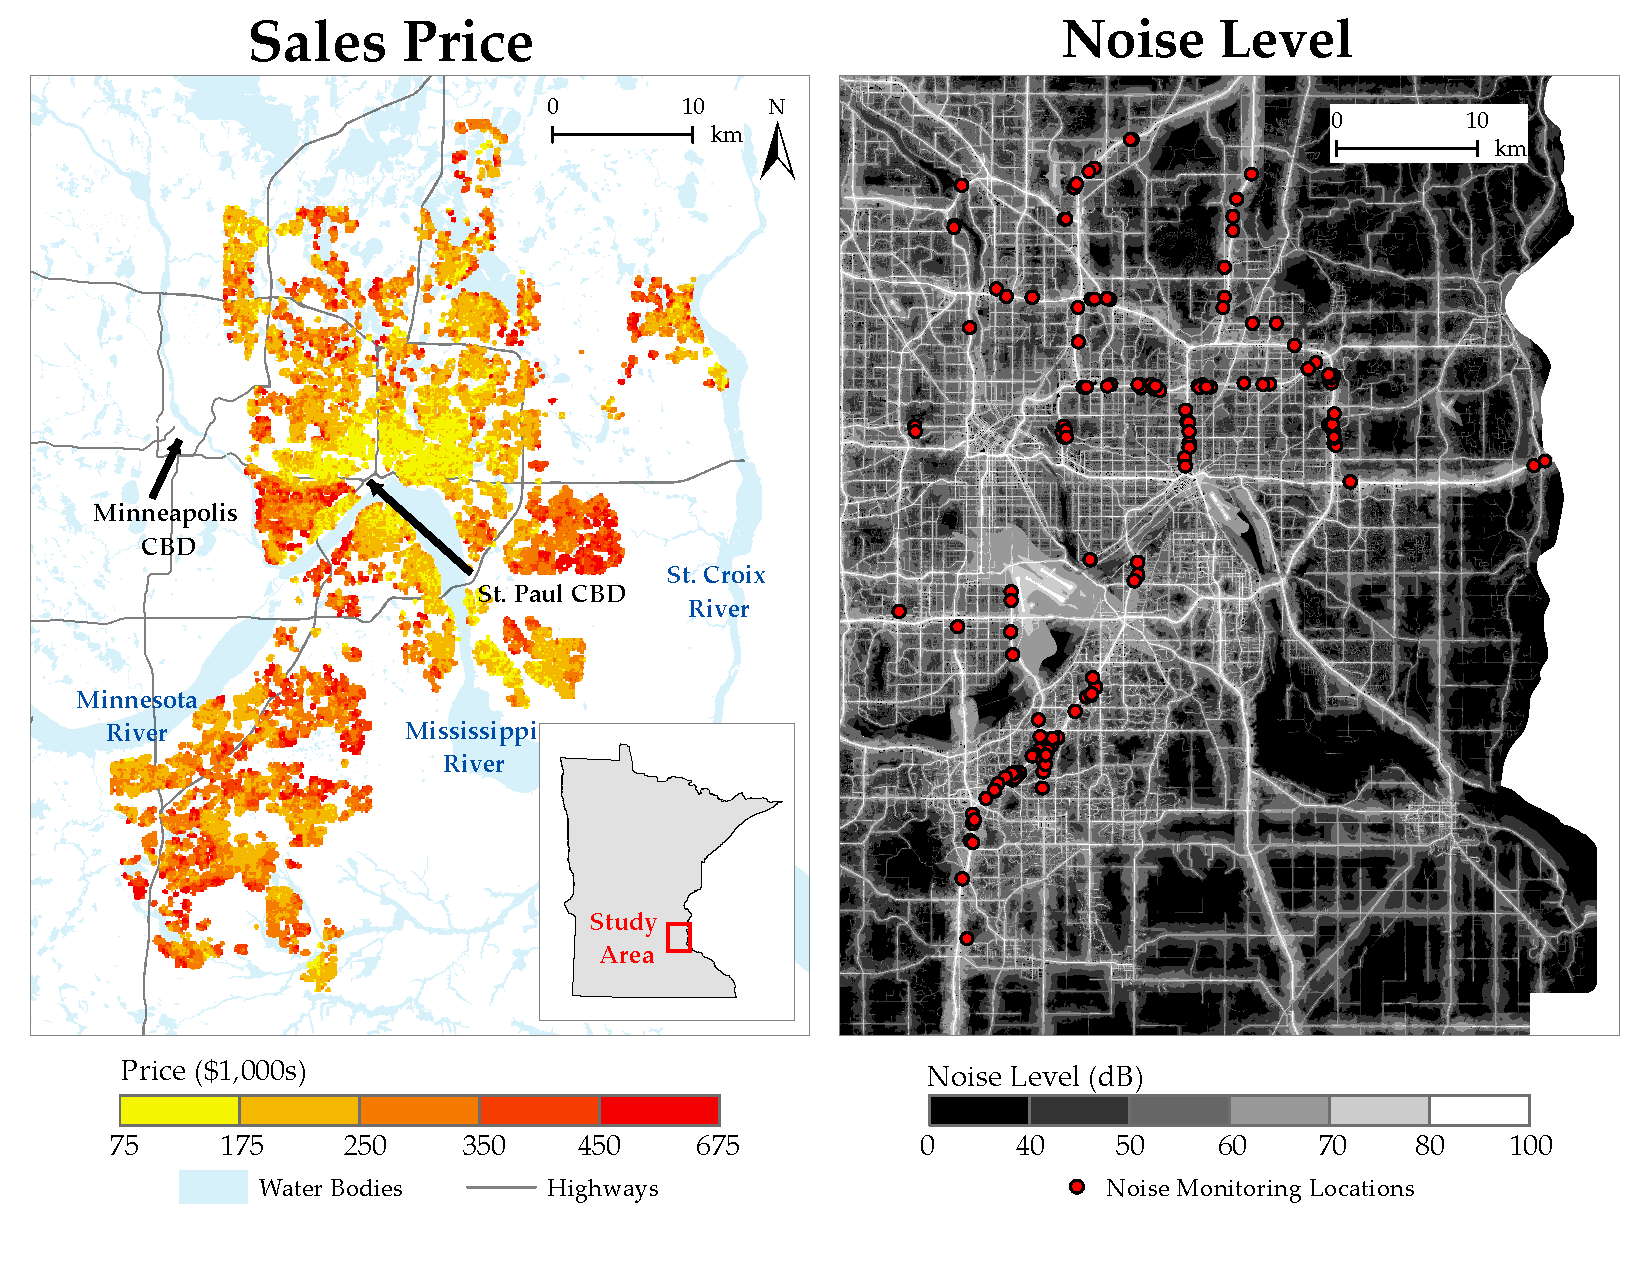
\includegraphics[width = 1.2\textwidth]{../graphs/Figure01}}
\caption{This figure shows the spatial extent of our study area, the significant spatial variation in single family house sales prices, as well as our noise data.}
\label{fig:overview}
\end{figure}

\begin{table}
\caption{Variable Description and Summary Statistics}
\label{tab:sumStats}
\makebox[\linewidth][c]{
\small
\begin{tabular}{lccccccc}
  \hline \hline
 & min & 25\% & 50\% & mean & 75\% & max & st dev \\ 
  \hline
Sale Price (\$1,000s) & 99 & 195 & 241 & 266 & 315 & 675 & 103 \\ \\
  Year House was Built & 1850 & 1950 & 1973 & 1967 & 1993 & 2010 & 32 \\ \\
  House Size (ft$^2$) & 390 & 1158 & 1628 & 1750 & 2189 & 4000 & 704 \\ \\
  Lot Size (acres) & 0.02 & 0.17 & 0.25 & 0.25 & 0.31 & 0.60 & 0.11 \\ \\
  Owner Occupancy (Yes = 1, No = 0) & 0.0 & 1.0 & 1.0 & 0.8 & 1.0 & 1.0 & 0.4 \\ \\
  Traffic Noise (dB) & 24.5 & 49.0 & 54.0 & 54.3 & 59.5 & 81.6 & 7.5 \\  \\
  Distance to Central Business District (km) & 1.1 & 6.8 & 13.2 & 14.7 & 21.8 & 37.1 & 8.9 \\ \\
  Distance to Nearest Park (km) & 0.0 & 1.1 & 2.2 & 2.6 & 3.8 & 9.7 & 1.9 \\ \\
  Distance to Nearest Lake (km) & 0.0 & 0.4 & 0.8 & 0.9 & 1.3 & 4.4 & 0.7 \\ \\
  Distance to Nearest Shopping Center (km) & 0.0 & 0.9 & 1.5 & 1.9 & 2.3 & 10.8 & 1.6 \\ \\
  Percent of Census Block Population Race = White & 0 & 80 & 90 & 85 & 96 & 100 & 17 \\ \\
  Percent of Census Block Population Under Age 18 & 0 & 21 & 27 & 27 & 33 & 67 & 9 \\ \\
  Median Income in Census Tract (\$1,000s) & 14 & 55 & 69 & 73 & 90 & 143 & 24 \\ \\
  Nearest Elementary School Test Scores & 336 & 360 & 365 & 364 & 370 & 552 & 11 \\ 
   \hline \hline
\end{tabular}
}
\end{table}

\begin{table}
\caption{Matrix of Pearson Correlation Coefficients for Quantitative Variables}\label{tab:cor}
\begin{center}
\small
\tabcolsep=0.05cm
\makebox[\linewidth][c]{
\begin{tabular}{l|rrrrrrrrrrrrr}
\hline \hline
 & \multicolumn{1}{x{.35in}}{Price} & \multicolumn{1}{x{.38in}}{House} & \multicolumn{1}{x{.35in}}{Lot} & 
 \multicolumn{1}{x{.35in}}{Built} & \multicolumn{1}{x{.35in}}{Noise} & \multicolumn{1}{x{.35in}}{CBD} & \multicolumn{1}{x{.35in}}{Park} & \multicolumn{1}{x{.35in}}{Lake} & \multicolumn{1}{x{.35in}}{Shop} & \multicolumn{1}{x{.35in}}{White} & 
 \multicolumn{1}{x{.35in}}{U18} & \multicolumn{1}{x{.35in}}{Inc.} & 
 \multicolumn{1}{x{.35in}}{Test} \\
  \hline
Sale Price & 1 &  &  &  &  &  &  &  &  &  &  &  &  \\ \\
House Size & 0.74 & 1 &  &  &  &  &  &  &  &  &  &  &  \\ \\
Lot Size  & 0.38 & 0.45 & 1 &  &  &  &  &  &  &  &  &  &  \\ \\
Year Built  & 0.45 & 0.52 & 0.47 & 1 &  &  &  &  &  &  &  &  &  \\ \\
Noise & -0.24 & -0.12 & -0.04 & -0.25 & 1 &  &  &  &  &  &  &  &  \\ \\
Distance to CBD  & 0.31 & 0.45 & 0.43 & 0.58 & -0.09 & 1 &  &  &  &  &  &  &  \\ \\
Distance to Park  & 0.25 & 0.28 & 0.22 & 0.42 & -0.17 & 0.57 & 1 &  &  &  &  &  &  \\ \\
Distance to Lake & -0.04 & -0.10 & -0.25 & -0.17 & -0.01 & -0.09 & 0.20 & 1 &  &  &  &  &  \\ \\
Distance to Shop  & 0.27 & 0.27 & 0.15 & 0.37 & -0.24 & 0.46 & 0.38 & 0.15 & 1 &  &  &  &  \\ \\
Percent White & 0.24 & 0.15 & 0.25 & 0.15 & -0.09 & 0.34 & 0.16 & -0.14 & 0.14 & 1 &  &  &  \\ \\
Percent Under 18 & 0.26 & 0.30 & 0.11 & 0.36 & -0.19 & 0.29 & 0.32 & 0.09 & 0.32 & -0.22 & 1 &  & \\  \\ 
Income & 0.52 & 0.50 & 0.41 & 0.57 & -0.24 & 0.53 & 0.38 & -0.12 & 0.36 & 0.35 & 0.32 & 1 &  \\ \\ 
Elem.\ Test Scores & 0.29 & 0.28 & 0.29 & 0.34 & -0.09 & 0.35 & 0.22 & -0.10 & 0.18 & 0.31 & 0.10 & 0.44 & 1 \\ \hline \hline 
\end{tabular} }
\end{center} 
\end{table}

\subsection*{Noise Data}
To determine the relationship between real estate prices and road traffic noise levels, we first created a traffic noise exposure surface by calculating the propagation of traffic noise over the landscape using the Federal Highway Authority (FHWA) 1978 standard \citep{Barry1978}. Methodological details of the process can be found in \citet{Nega2012} and \citet{Nega2013}. Here we provide a brief summary. 

The modeling of traffic noise has three key components: choosing the mathematical function for noise propagation, assembling the input data, and assessing the accuracy of the model prediction. We used the FHWA 1978 standard model for calculating the noise level because it is currently used by the state of Minnesota.  According to this standard, the noise level at any given location on the landscape can be expressed:  
\begin{eqnarray}\label{eq:noise}
L_{EQ}(i) &=& \bar{L}_0(i) + 0.115 \sigma _i^2 + 10 log \frac{N_i \pi D_0}{T*S_i} + 10 log \left[ \frac{D_0}{D}\right]^{1 + \alpha}  \nonumber \\
&& + 10 log \left( \frac{\psi _{\alpha (\phi _1, \phi _2)}}{\pi}\right) + \Delta _{gradient} + \Delta _{shielding}
\end{eqnarray}
where 
\begin{itemize}
\item[] $L_{EQ}(i)$ is A-weighted hourly energy equivalent noise level in decibels (dBA), which is calculated for each class $i$ of vehicle (automobile and trucks); 
\item[] $\bar{L}_0(i)$ is the mean Sound Pressure Level (SPL) at the reference distance for class $i$; \item[] $\sigma _i$ is the standard deviation of the SPL for each class of vehicle; 
\item[] $N_i$ is the number of vehicles of the $i^{th}$ class passing during the relevant hour; 
\item[] $D_0$ is the reference distance (usually 15 m); 
\item[] $D$ is the perpendicular distance from the road center line to the receiver; 
\item[] $\alpha$ is a site parameter (soft and hard surface), $0 < \alpha < 1$; 
\item[] $S_i$ is the mean speed of the $i^{th}$ class; 
\item[] $T$ is the duration, usually 1 hour; 
\item[] $\phi _1$ and $\phi _2$ are the angles from the perpendicular of the limits of the observer's view of a section of the road. They are used to account for only the energy coming from a portion of the roadway; 
\item[] $\Delta _{gradient}$ is an adjustment for road surface gradient; and 
\item[] $\Delta _{shielding}$ is a shielding adjustment (land cover, buildings, noise barriers).
\end{itemize}

We used the SoundPlan\texttrademark noise modeling software to implement equation~\ref{eq:noise} using several data sources as inputs.  A 2007 road centerline and the associated traffic characteristics (volume and proportion of trucks and vehicles) for the region were obtained from the Minnesota Department of Transportation (MNDoT).  We converted the posted speed of each road segment into a GIS layer.  We used three data sources for the shielding adjustment: buildings, foliage, and noise barriers.  We extracted the perimeter and height of 818,500 buildings using a combination of LiDAR data and aerial photography.  Foliage shielding was accounted for by extracting forest polygons that are at least 10 m high and have an area $\geq$10,000 m$^2$ from a 2005 land use and 2001 National Land Cover Data. We obtained a noise barrier layer from the MNDoT containing the locations, width, and height of each noise barriers to account for its shielding effect. 

In order to incorporate noise produced by aircraft into the overall noise exposure, we obtained the aircraft noise contour lines of the region from the Twin Cities Metropolitan Airports Commission. The contour line noise values coincident with the traffic noise surface were then added following rules of logarithmic addition. For example, adding 52 dBA from aircraft contour line into the noise surface where the noise value was 51 dBA yielded 53.5 dBA. 

Predicted noise output was calculated at a grid resolution of 10 m$^2$.  We conducted a validation of the model output by comparing it with observed noise levels, which were sampled at 134 locations along a major highway. The relationship between the mean observed and predicted noise levels was found to be linear and moderately strong with a correlation of 0.76. A map of our noise surface and the validation sites can be seen in Figure~\ref{fig:overview}. Once the noise surface for the entire region was developed, we extracted the noise surface for the present study by overlaying the housing parcel boundaries and calculating the mean noise level within the parcel. 

\subsection*{House Structural Attributes}\label{structural}
According to a review by \cite{Wilhelmsson2000}, the five most common structural attributes included in real estate hedonic pricing studies are living area, number of bathrooms, age, garage and lot size.  The 2010 MetroGIS Regional Parcel Dataset includes structural data on living area, age, garage presence, lot size, owner-occupancy and house architectural style for every transaction. However, standard additional control variables like the number of bathrooms, bedrooms, and size of garage were not available through this source. We were able to obtain additional data for the number of bedrooms, bathrooms, and size of the garage for a subset of our house sales from the Dakota County Assessor's Office. In section \ref{Discussion} we show that the inclusion of these variables in our model does not significantly change our results for these areas. Therefore, we feel confident in our results even without these independent variables for most of our study area.

\subsection*{Other Locational Attributes}
A common real estate adage states that the three most important real estate attributes are: location, location and location. Knowing where each house is located allowed us to construct a vector of other attributes associated with the sales transaction. Using GIS software we calculated the Euclidean distance to numerous points of interest within the dataset, such as the nearest central business district, shopping centers, parks, and lakes. Additionally, three local demographic variables denoting the median household income for the surrounding census tract, the percentage of the population that identified their race as ``white'', and the percentage of the population that is under the age of 18 (both at the census block group level) were created through the use of TIGER shapefiles from the 2010 Census Bureau and data from the 2010 American Community Survey. Lastly, we associated each transaction with its nearest elementary school and included the average 3rd grade Minnesota Comprehensive Assessment (MCA) score for the local elementary school during the year of purchase.\footnote{Test scores were obtained from the Minnesota Department of Education website. The school district and elementary school attendance boundary spatial information were obtained from the Minnesota Geospatial Information Office Clearinghouse Data Catalog.} 

\subsection*{Time}
Due to concerns of sample selection bias before, during, and after the economic recession, we compared the characteristics of our data by year to look for important differences. Table \ref{tab:SumStatsTime} displays the mean variable values by year of sale. The mean sale price in 2009 (roughly \$230,000) was almost 20 percent lower than the mean sale price in 2006 (roughly \$280,000). However, most other variable means show small or no differences across years.\footnote{We also created univariate density plots of the variables by year to check for differences in the shape and spread of the distributions over time. With the exception of house prices, we found no differences in the variable distributions over time. Figures available upon request.} We also mapped the locations of sales transactions to check for differences in geographic dispersion of sales over time, but found none (see Figure~\ref{fig:SalesYear}). Thus, with the exception of lower sales prices in later years, house characteristics in our sample appear similar before, during, and after the economic recession. Of course, it is still possible that the houses differed over time in unobserved characteristics.

\begin{table}
\caption{Mean Variable Values by Year}\label{tab:SumStatsTime}
\makebox[\textwidth][c]{
\scriptsize
  \centering
    \begin{tabular}{lcccccc|c}
    \\[-1.8ex]\hline 
\hline \\[-1.8ex] 
    & \multicolumn{6}{c}{Year of House Sale} & \\
    Variable & 2005 & 2006 & 2007 & 2008 & 2009 & 2010 & \multicolumn{1}{r}{All Years}\\ \hline 
Sale Price (\$1,000s) & 279 & 282 & 275 & 262 & 231 & 233 & 266 \\ \\
  Year House was Built & 1967 & 1966 & 1966 & 1971 & 1968 & 1968 & 1967 \\ \\
  House Size (feet$^2$) & 1737 & 1736 & 1743 & 1813 & 1727 & 1775 & 1750 \\ \\
  Lot Size (acres) & 0.25 & 0.25 & 0.25 & 0.26 & 0.25 & 0.26 & 0.25 \\ \\
  Owner Occ (Y = 1, N = 0) & 0.87 & 0.87 & 0.92 & 0.86 & 0.60 & 0.77 & 0.83 \\ \\
  Traffic Noise (dB) & 54.4 & 54.5 & 54.6 & 53.7 & 54.0 & 54.0 & 54.3 \\ \\
  Dist CBD (km) & 14.7 & 14.6 & 14.8 & 15.0 & 14.3 & 14.5 & 14.7 \\ \\
  Dist to  Park (km) & 2.6 & 2.6 & 2.6 & 2.8 & 2.6 & 2.6 & 2.6 \\ \\
  Dist to Lake (km) & 0.9 & 0.9 & 0.9 & 0.9 & 0.9 & 0.9 & 0.9 \\ \\
  Dist to  Shop (km) & 1.9 & 1.9 & 1.8 & 2.0 & 1.9 & 1.9 & 1.9 \\ \\
  Percent Race = White & 84 & 84 & 85 & 86 & 85 & 86 & 85 \\ \\
  Percent Under Age 18 & 28 & 28 & 27 & 28 & 27 & 27 & 27 \\ \\
  Income (\$1,000s) & 72 & 72 & 72 & 75 & 73 & 73 & 73 \\ \\
  Elementary Test Scores & 365 & 365 & 365 & 364 & 362 & 366 & 364 \\  \hline
  Number of Observations &  10,990  & 8,885  &  6,549  & 5,498  &  5,961  & 4,200  & 42,083  \\ \hline \hline
    \end{tabular}%
}
\end{table}

\begin{figure}
\makebox[\textwidth][c]{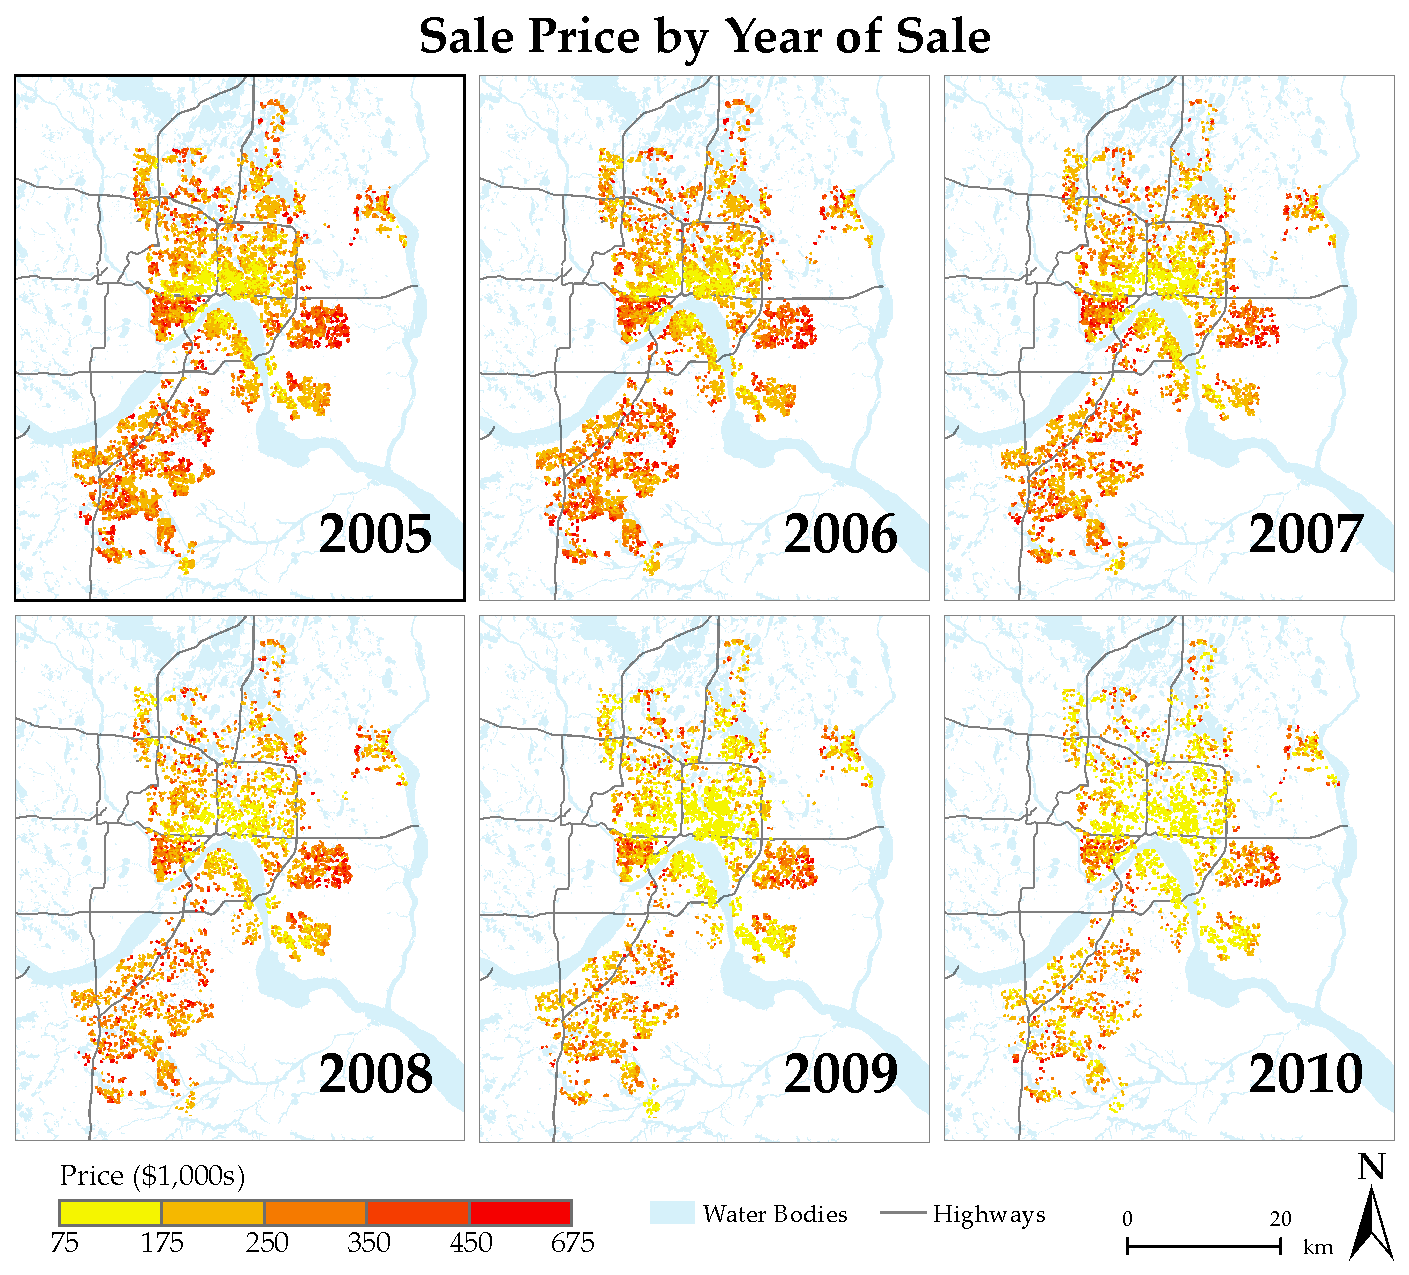
\includegraphics[width = \textwidth]{../graphs/Figure02}}
\caption{This figure shows the spatial distribution of observed sales prices over time. The change in color from 2005 to 2010 denotes the drop in sales prices associated with the recession of 2008-09. There are clear spatial patterns in  house prices that persist over time (locations with relatively high vs. low prices in one year tend to be the same in other years). However, we see no evidence that sales shifted from one area of our study region to another (neighborhoods with many sales in 2005 also tend to have many sales in 2010). }
\label{fig:SalesYear}
\end{figure}

\section{Basic Econometric Model}\label{basicModel}
Consistent with past research, this study estimates a semi-logarithmic hedonic price function.  Before implementing the Locally Weighted Regression model, we present the results of a simpler econometric model given by equation~\eqref{eq:model}.
\begin{equation}\label{eq:model}	
ln \textrm{ Sale Price}_i = \beta _0 + \beta _1 \textrm{Noise}_i+ \beta _2 S_i+ \beta _3 N_i + \beta _4 T_i + \textrm{error}_i
\end{equation}
Noise$_i$ is the noise level for house $i$, $S_i$ is a vector of the house's structural attributes, $N_i$ is a vector of the neighborhood attributes, and $T_i$ is a vector of time fixed effects. Model (A) in Table \ref{tab:globalRegression} displays the results of this basic Ordinary Least Squares regression model. In addition to the important structural and neighborhood variables, we also included fixed effects for each city and an interaction term between month and year of sale.\footnote{We'd like to thank an anonymous referee for suggesting this interaction fixed effect specification as a means of controlling for government policies like the First-Time Homebuyer Tax Credit that also may have affected the sales price of houses during our study period. } The traffic noise coefficient suggests houses in our data that are similar in all respects but a one decibel difference in noise will, on average, have sales prices roughly 0.27 percent lower at the noisier location. 

\begin{table}
\caption{Basic Global Regression Results}
\label{tab:globalRegression}
\makebox[\textwidth][c]{
\scriptsize
  \centering
\begin{tabular}{@{\extracolsep{-1pt}}lD{.}{.}{-4} D{.}{.}{-4} D{.}{.}{-4} D{.}{.}{-4} } 
\\[-1.8ex]\hline 
\hline \\[-1.8ex] 
 & \multicolumn{4}{c}{\textit{Dependent variable: ln Sale Price}} \\ 
\cline{2-5} \\[-1.8ex] 
& \multicolumn{1}{r}{Model (A)} & \multicolumn{1}{r}{Model (B)} & \multicolumn{1}{r}{Model (C)} & \multicolumn{1}{r}{Model (D)}\\ 
& \multicolumn{1}{r}{All Years} & \multicolumn{1}{r}{Year=2006} & \multicolumn{1}{r}{Year=2008} & \multicolumn{1}{r}{Year=2010}\\
\hline \\[-1.8ex] 
Noise (dB) & -0.0027^{***} & -0.0020^{***} & -0.0033^{***} & -0.0040^{***} \\ 
  & (0.0001) & (0.0003) & (0.0005) & (0.0006) \\ 
  & & & & \\ 
 House Size (1,000s ft$^2$) & 0.2914^{***} & 0.2847^{***} & 0.2810^{***} & 0.3066^{***} \\ 
  & (0.0022) & (0.0043) & (0.0067) & (0.0084) \\ 
  & & & & \\ 
 Lot Size (acres) & 0.2493^{***} & 0.2719^{***} & 0.2799^{***} & 0.2135^{***} \\ 
  & (0.0118) & (0.0221) & (0.0359) & (0.0447) \\ 
  & & & & \\ 
 Owner Occupancy Dummy & 0.0222^{***} & -0.0027 & 0.0478^{***} & 0.0298^{***} \\ 
  & (0.0026) & (0.0050) & (0.0085) & (0.0097) \\ 
  & & & & \\ 
 Year House Built & 0.0020^{***} & 0.0025^{***} & 0.0018^{***} & 0.0011^{***} \\ 
  & (0.0001) & (0.0001) & (0.0002) & (0.0002) \\ 
  & & & & \\ 
 Percent Under Age 18 & -0.0001 & 0.00002 & -0.0002 & -0.0006 \\ 
  & (0.0001) & (0.0002) & (0.0004) & (0.0005) \\ 
  & & & & \\ 
 Percent White & 0.0037^{***} & 0.0031^{***} & 0.0040^{***} & 0.0040^{***} \\ 
  & (0.0001) & (0.0001) & (0.0002) & (0.0003) \\ 
  & & & & \\ 
 Median Income (\$1,000s) & 0.0023^{***} & 0.0021^{***} & 0.0023^{***} & 0.0029^{***} \\ 
  & (0.0001) & (0.0001) & (0.0002) & (0.0003) \\ 
  & & & & \\ 
 Elementary Test Scores & 0.0009^{***} & 0.0023^{***} & 0.0040^{***} & 0.0001 \\ 
  & (0.0001) & (0.0003) & (0.0005) & (0.0002) \\ 
  & & & & \\ 
 Dist to CBD (km) & 0.0078^{***} & 0.0083^{***} & 0.0053^{***} & 0.0101^{***} \\ 
  & (0.0005) & (0.0010) & (0.0016) & (0.0020) \\ 
  & & & & \\ 
 Dist to Lake (km) & 0.0230^{***} & 0.0246^{***} & 0.0021 & 0.0343^{***} \\ 
  & (0.0017) & (0.0032) & (0.0054) & (0.0067) \\ 
  & & & & \\ 
 Dist to Park (km) & 0.0014 & -0.0027 & 0.0099^{***} & 0.0064^{*} \\ 
  & (0.0009) & (0.0017) & (0.0027) & (0.0034) \\ 
  & & & & \\ 
 Dist to Shop (km) & -0.0019^{*} & -0.0020 & -0.0063^{*} & -0.0020 \\ 
  & (0.0010) & (0.0019) & (0.0033) & (0.0041) \\ 
  & & & & \\ 
\hline \\[-1.8ex] 
Home Style Fixed Effects & \multicolumn{1}{c}{Yes} & \multicolumn{1}{c}{Yes} & \multicolumn{1}{c}{Yes} & \multicolumn{1}{c}{Yes} \\ 
Month*Year Fixed Effects & \multicolumn{1}{c}{Yes} & \multicolumn{1}{c}{Yes} & \multicolumn{1}{c}{Yes} & \multicolumn{1}{c}{Yes} \\ 
City Fixed Effects & \multicolumn{1}{c}{Yes} & \multicolumn{1}{c}{Yes} & \multicolumn{1}{c}{Yes} & \multicolumn{1}{c}{Yes} \\ 
\hline \\[-1.8ex] 
Observations & \multicolumn{1}{c}{42,083} & \multicolumn{1}{c}{8,885} & \multicolumn{1}{c}{5,498} & \multicolumn{1}{c}{4,200} \\ 
R$^{2}$ & \multicolumn{1}{c}{0.742} & \multicolumn{1}{c}{0.785} & \multicolumn{1}{c}{0.691} & \multicolumn{1}{c}{0.668} \\ 
\hline 
\hline \\[-1.8ex] 
\multicolumn{5}{l}{Note: (Standard errors) and $^{*}$p$<$0.1; $^{**}$p$<$0.05; $^{***}$p$<$0.01} \\ 
\end{tabular} 
}
\end{table}

Further exploratory analysis suggests the assumption of temporal and geographic stationarity of the hedonic price function is inappropriate. We first tested for temporal changes in the coefficients for house size, lot size, and noise by creating interaction terms between these variables and the month*year fixed effects. In all three cases the improved model fit was significantly more than expected due to random chance. Columns (B)--(D) of Table~\ref{tab:globalRegression} show the results of re-estimating model (A) using only sales within three separate years of data to allow all coefficients to vary over time. Subsequent work with models (B)--(D) also suggested that many of the important regression coefficients vary across the different cities within our sample. We rejected the null hypothesis that interaction terms between cities and house size, lot size, noise, etc. are zero.\footnote{Results of specific hypothesis tests are available upon request.}  These results should be taken with appropriate skepticism, as the models are simple Ordinary Least Squares regressions and the spatial and temporal nature of the data likely violate assumptions of the Classical Linear Regression Model. However, the initial findings suggest the relationship between house prices and many other hedonic characteristics in our data vary over space and time. 

While methods exist for parameterizing variation in the hedonic function \citep[such as spatial expansion as suggested by][]{Casetti1972}, we have no a priori knowledge of how to parameterize the variation and therefore turn to a semi-parametric form of hedonic regression estimation. This flexible modeling approach lets the data reveal how relationships vary, rather than requiring the researcher to specify them beforehand. 

\section{Locally Weighted Regression Model}
Locally Weighted Regression (LWR) techniques are described in detail by \citet{Cleveland1988} and use weighted least squares to estimate regression coefficients as a function of the local data. \citet{Brunsdon1998b}, \citet{Fotheringham2002}, and others have since popularized the application of LWR in a geographic context (referring to the technique as Geographically Weighted Regression). The basic formulation can be described in equation \eqref{eq:LWRbeta}, 
\begin{equation}\label{eq:LWRbeta}
\hat{\beta}_i = (X'W_iX)^{-1}X'W_iY,
\end{equation}
where X is a $n \times m$ matrix of independent variables, $W_i$ is the $n \times n$ weights matrix, and Y is the $n \times 1$ vector of dependent variable values. The weights matrix, $W_i$ is a diagonal matrix where element $w_{jj}$ denotes the weight that the $j^{th}$ data point will receive in the regression coefficients estimated at location $i$ in the dataset. We employ a bi-square weights function and a k-nearest neighbor bandwidth approach as described in equation~\eqref{eq:weights}, 
\begin{equation}\label{eq:weights}
w_{jj}=\left[1-\left(\frac{d_{ij}}{d_{k}}\right)^2 \right]^2 \textrm{ if  }d_{ij}<d_{ik}\textrm{, otherwise = 0},
\end{equation}
where $d_{ij}$ denotes the distance between observations $i$ and $j$, and $d_{ik}$ is the distance from observation $i$ to the $k^{th}$ nearest observation. This function assigns weights close to 1 for data points near observation $i$, weights positive but closer to zero for observations farther away, and zero for all $n-k$ observations farther away than the $k^{th}$ nearest observation. We estimate LWR coefficients using bandwidths ranging from as small as $k=100$ observations and as large as 4,000 observations. 

We measure the LWR model fit by calculating the Generalized Cross Validation score as detailed in equation~\eqref{eq:GCV},
\begin{equation}\label{eq:GCV}
n*\sum_{i=1}^{n}\frac{(y_i-\hat{y}_i)^2}{(n-v_1)^2}, 
\end{equation} 
where $y_i$ is the dependent variable value, $\hat{y}_i$ is the predicted dependent variable value for observation $i$, and $v_1$ is the ``effective number of model parameters.'' The value  
$v_1=$tr(\textbf{S}), where the matrix \textbf{S} is the ``hat matrix'' which maps $y$ onto $\hat{y}$,
                   \begin{equation*}
                   \hat{y}=\textbf{S}y,
                   \end{equation*}
                   and each row of \textbf{S}, $r_i$ is given by:
                     \begin{equation*}
                   r_i=X_i(X'W_iX)^{-1}X'W_i.
                   \end{equation*}
The GCV score is a convenient model selection metric that rewards models that provide a good fit to the data, while penalizing models with a greater number of model parameters \citep{Loader1999, McMillen2010}. Model selection via this strategy has been shown to discern whether spatially varying relationships exist, accurately estimate spatially varying coefficients, even outperform other spatial econometric techniques, and do so without wasting degrees of freedom \citep{Paez2011, McMillen2010, McMillen2012}. 

%\section{Results}
Similar to the basic econometric model described in Section \ref{basicModel}, we estimated the LWR model with logged sales price as a function of structural and neighborhood variables, location and time. In order to account for changing market conditions over time, when estimating the LWR model for a particular observation in our data, we used only houses sold within the past 12 months and also included month fixed effects to account for seasonality and other policy changes such as tax credits for home purchases. Thus, the coefficient estimates at a particular house were estimated using data from other sales nearby in both time and geography.

\subsection*{Improved Model Performance}
The use of the Locally Weighted Regression model significantly improved model performance. Figure \ref{fig:GCVmodel} displays the GCV score for three different model specifications estimated at the ``global'' level as well as with varying numbers of observations included in the regression bandwidth. We estimated three different hedonic function specifications with different levels of additional spatial control variables. Model (1) included the noise variable, the basic structural characteristics (size of the house in square feet, size of the lot in acres, a categorical variable denoting the architectural style of the house, and whether or not the house is owner-occupied) plus month of sale*year fixed effects. Model (2) added neighborhood and locational variables (test scores at the local elementary school, census tract median income, percent of the census block population that is white, percentage of the census block that is under age 18 and distances to the central business district, nearest park, nearest shopping center, and nearest lake). Model (3) added city fixed effects to Model (2), thus explicitly including both common important characteristics of neighborhood quality while also allowing for spatial heterogeneity in the regression coefficients, and even city-level fixed effects to control for omitted variables that vary at the municipal level.

Two important conclusions can be drawn from these results. First, local analyses performed significantly better than global models. All three models have significantly lower GCV scores across a range of local bandwidths compared to their global counterparts. Secondly, even conditional on having performed local analysis, adding additional explanatory neighborhood and locational variables still improved model fit. Overall, Model (3) consistently outperformed the other two models-- albeit only slightly better than Model (2). The minimum GCV score was obtained using a bandwidth of 500 nearest houses and a model including structural, neighborhood, and locational variables in addition to time and city fixed-effects. 

\begin{figure}
  \makebox[\textwidth][c]{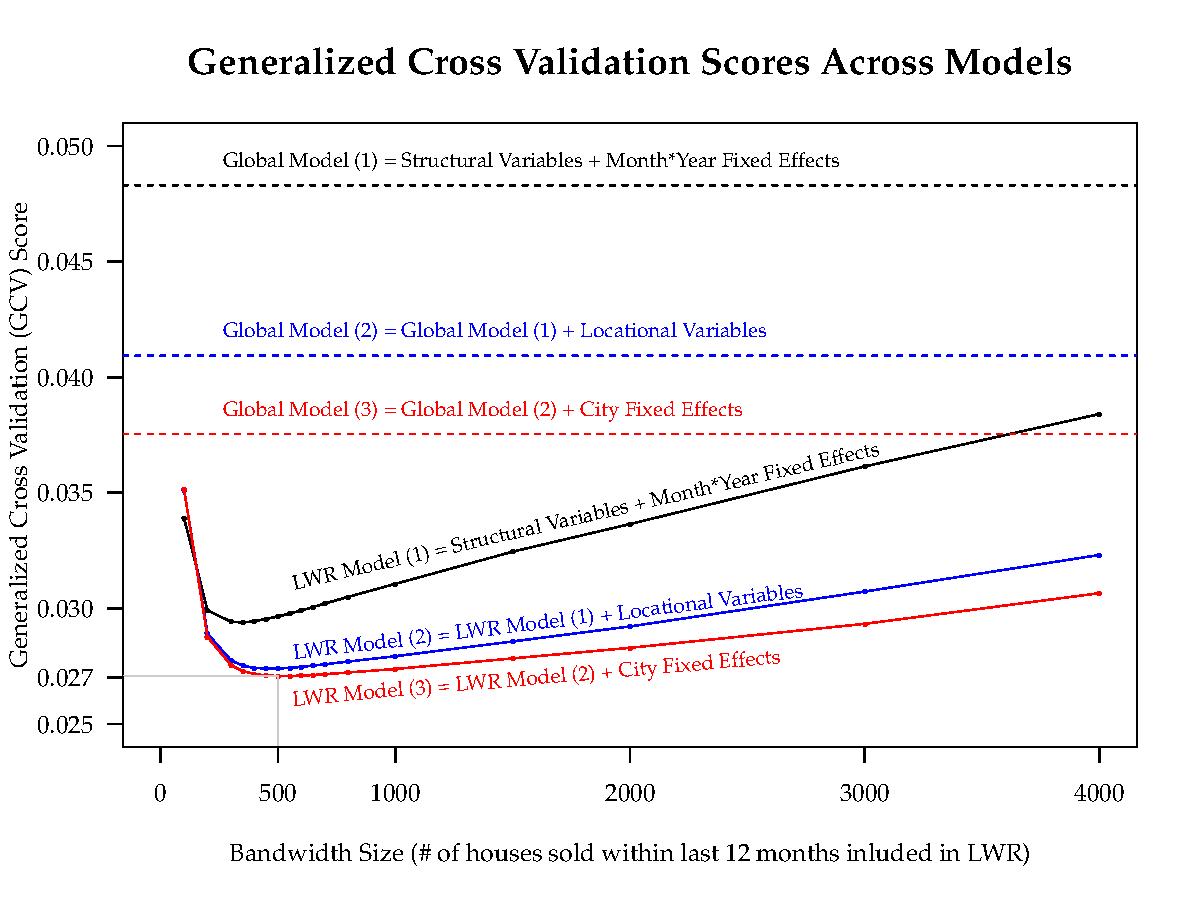
\includegraphics[width = 1.2\textwidth]{../graphs/Figure03}}
\caption{This figure shows the relationship between bandwidth size and the GCV score for three different Locally Weighted Regression (LWR) models. For comparison, the GCV scores for each model when estimated at a global scale are also shown. Note that the LWR models all have significantly smaller GCV scores than the global models. The minimum GCV score is obtained by LWR Model (3) at a bandwidth of 500 nearest houses.}
\label{fig:GCVmodel}
\end{figure}


\begin{table}[!htbp]   
  \caption{\mbox{LWR Coefficient Mean and (10$^{th}$ to 90$^{th}$ Percentile) Values for Selected Bandwidths} }
  \label{tab:LWR} 
  \makebox[\textwidth][c]{
\scriptsize
  \centering
\begin{tabular}{@{\extracolsep{-1pt}} D{.}{.}{4} D{.}{.}{4} D{.}{.}{4} D{.}{.}{4} D{.}{.}{4} } 
\\[-1.8ex]\hline 
\hline \\[-1.8ex] 
& \multicolumn{4}{c}{Dependent Variable = ln(Sales Price)} \\ \\
 & \multicolumn{1}{c}{Nearest 500 sales\ding{105}} & \multicolumn{1}{c}{Nearest 650 sales} & \multicolumn{1}{c}{Nearest 1,000 sales} & \multicolumn{1}{c}{Nearest 2,000 sales} \\ \hline \\
\multicolumn{1}{l}{Noise (dB)} & \multicolumn{1}{c}{-0.0034} & \multicolumn{1}{c}{-0.0034} & \multicolumn{1}{c}{-0.0033} & \multicolumn{1}{c}{-0.0032} \\ 
\multicolumn{1}{c}{} & \multicolumn{1}{c}{(-0.0064 to -0.0007)} & \multicolumn{1}{c}{(-0.0061 to -0.0009)} & \multicolumn{1}{c}{(-0.0057 to -0.0013)} & \multicolumn{1}{c}{(-0.0049 to -0.0017)} \\ 
\multicolumn{1}{c}{} & \multicolumn{1}{c}{} & \multicolumn{1}{c}{} & \multicolumn{1}{c}{} & \multicolumn{1}{c}{} \\ 
\multicolumn{1}{l}{House Size (1,000s ft$^2$)} & \multicolumn{1}{c}{0.27} & \multicolumn{1}{c}{0.27} & \multicolumn{1}{c}{0.27} & \multicolumn{1}{c}{0.28} \\ 
\multicolumn{1}{c}{} & \multicolumn{1}{c}{(0.18 to 0.39)} & \multicolumn{1}{c}{(0.19 to 0.39)} & \multicolumn{1}{c}{(0.20 to 0.40)} & \multicolumn{1}{c}{(0.20 to 0.37)} \\ 
\multicolumn{1}{c}{} & \multicolumn{1}{c}{} & \multicolumn{1}{c}{} & \multicolumn{1}{c}{} & \multicolumn{1}{c}{} \\ 
\multicolumn{1}{l}{Lot Size (acres)} & \multicolumn{1}{c}{0.42} & \multicolumn{1}{c}{0.42} & \multicolumn{1}{c}{0.42} & \multicolumn{1}{c}{0.40} \\ 
\multicolumn{1}{c}{} & \multicolumn{1}{c}{(0.17 to 0.73)} & \multicolumn{1}{c}{(0.19 to 0.71)} & \multicolumn{1}{c}{(0.21 to 0.67)} & \multicolumn{1}{c}{(0.25 to 0.58)} \\ 
\multicolumn{1}{c}{} & \multicolumn{1}{c}{} & \multicolumn{1}{c}{} & \multicolumn{1}{c}{} & \multicolumn{1}{c}{} \\ 
\multicolumn{1}{l}{Year House Built} & \multicolumn{1}{c}{0.0046} & \multicolumn{1}{c}{0.0045} & \multicolumn{1}{c}{0.0043} & \multicolumn{1}{c}{0.0038} \\ 
\multicolumn{1}{c}{} & \multicolumn{1}{c}{(0.0004 to 0.010)} & \multicolumn{1}{c}{(0.0005 to 0.0096)} & \multicolumn{1}{c}{(0.0005 to 0.0090)} & \multicolumn{1}{c}{(0.0004 to 0.0080)} \\ 
\multicolumn{1}{c}{} & \multicolumn{1}{c}{} & \multicolumn{1}{c}{} & \multicolumn{1}{c}{} & \multicolumn{1}{c}{} \\ 
\multicolumn{1}{l}{Owner Occupancy} & \multicolumn{1}{c}{0.023} & \multicolumn{1}{c}{0.024} & \multicolumn{1}{c}{0.023} & \multicolumn{1}{c}{0.021} \\ 
\multicolumn{1}{c}{} & \multicolumn{1}{c}{(-0.029 to 0.080)} & \multicolumn{1}{c}{(-0.024 to 0.076)} & \multicolumn{1}{c}{(-0.018 to 0.068)} & \multicolumn{1}{c}{(-0.012 to 0.056)} \\ 
\multicolumn{1}{c}{} & \multicolumn{1}{c}{} & \multicolumn{1}{c}{} & \multicolumn{1}{c}{} & \multicolumn{1}{c}{} \\ 
\multicolumn{1}{l}{Percent White} & \multicolumn{1}{c}{0.0012} & \multicolumn{1}{c}{0.0013} & \multicolumn{1}{c}{0.0014} & \multicolumn{1}{c}{0.0016} \\ 
\multicolumn{1}{c}{} & \multicolumn{1}{c}{(-0.0003 to 0.0029)} & \multicolumn{1}{c}{(-0.0001 to 0.0028)} & \multicolumn{1}{c}{(0.0001 to 0.0028)} & \multicolumn{1}{c}{(0.0003 to 0.0032)} \\ 
\multicolumn{1}{c}{} & \multicolumn{1}{c}{} & \multicolumn{1}{c}{} & \multicolumn{1}{c}{} & \multicolumn{1}{c}{} \\ 
\multicolumn{1}{l}{Percent Under Age 18} & \multicolumn{1}{c}{0.00047} & \multicolumn{1}{c}{0.00045} & \multicolumn{1}{c}{0.00040} & \multicolumn{1}{c}{0.00034} \\ 
\multicolumn{1}{c}{} & \multicolumn{1}{c}{(-0.0016 to 0.0025)} & \multicolumn{1}{c}{(-0.0014 to 0.0022)} & \multicolumn{1}{c}{(-0.0011 to 0.0019)} & \multicolumn{1}{c}{(-0.0008 to 0.0015)} \\ 
\multicolumn{1}{c}{} & \multicolumn{1}{c}{} & \multicolumn{1}{c}{} & \multicolumn{1}{c}{} & \multicolumn{1}{c}{} \\ 
\multicolumn{1}{l}{Median Income (\$1,000s)} & \multicolumn{1}{c}{0.0006} & \multicolumn{1}{c}{0.0008} & \multicolumn{1}{c}{0.0010} & \multicolumn{1}{c}{0.0014} \\ 
\multicolumn{1}{c}{} & \multicolumn{1}{c}{(-0.0014 to 0.0033)} & \multicolumn{1}{c}{(-0.0010 to 0.0033)} & \multicolumn{1}{c}{(-0.0006 to 0.0037)} & \multicolumn{1}{c}{(-0.0002 to 0.0042)} \\ 
\multicolumn{1}{c}{} & \multicolumn{1}{c}{} & \multicolumn{1}{c}{} & \multicolumn{1}{c}{} & \multicolumn{1}{c}{} \\ 
\multicolumn{1}{l}{Elementary Test Scores} & \multicolumn{1}{c}{-0.00002} & \multicolumn{1}{c}{0.00008} & \multicolumn{1}{c}{0.00029} & \multicolumn{1}{c}{0.00044} \\ 
\multicolumn{1}{c}{} & \multicolumn{1}{c}{(-0.0056 to 0.0055)} & \multicolumn{1}{c}{(-0.0050 to 0.0049)} & \multicolumn{1}{c}{(-0.0040 to 0.0042)} & \multicolumn{1}{c}{(-0.0025 to 0.0037)} \\ 
\multicolumn{1}{c}{} & \multicolumn{1}{c}{} & \multicolumn{1}{c}{} & \multicolumn{1}{c}{} & \multicolumn{1}{c}{} \\ 
\multicolumn{1}{l}{Distance to Lake (km)} & \multicolumn{1}{c}{-0.0150} & \multicolumn{1}{c}{-0.0110} & \multicolumn{1}{c}{-0.0076} & \multicolumn{1}{c}{-0.0051} \\ 
\multicolumn{1}{c}{} & \multicolumn{1}{c}{(-0.091 to 0.058)} & \multicolumn{1}{c}{(-0.077 to 0.055)} & \multicolumn{1}{c}{(-0.063 to 0.052)} & \multicolumn{1}{c}{(-0.048 to 0.043)} \\ 
\multicolumn{1}{c}{} & \multicolumn{1}{c}{} & \multicolumn{1}{c}{} & \multicolumn{1}{c}{} & \multicolumn{1}{c}{} \\ 
\multicolumn{1}{l}{Distance to Park (km)} & \multicolumn{1}{c}{-0.011} & \multicolumn{1}{c}{-0.011} & \multicolumn{1}{c}{-0.009} & \multicolumn{1}{c}{-0.002} \\ 
\multicolumn{1}{c}{} & \multicolumn{1}{c}{(-0.060 to 0.033)} & \multicolumn{1}{c}{(-0.049 to 0.025)} & \multicolumn{1}{c}{(-0.037 to 0.016)} & \multicolumn{1}{c}{(-0.018 to 0.011)} \\ 
\multicolumn{1}{c}{} & \multicolumn{1}{c}{} & \multicolumn{1}{c}{} & \multicolumn{1}{c}{} & \multicolumn{1}{c}{} \\ 
\multicolumn{1}{l}{Distance to Shop (km)} & \multicolumn{1}{c}{0.0092} & \multicolumn{1}{c}{0.0096} & \multicolumn{1}{c}{0.0100} & \multicolumn{1}{c}{0.0078} \\ 
\multicolumn{1}{c}{} & \multicolumn{1}{c}{(-0.033 to 0.052)} & \multicolumn{1}{c}{(-0.027 to 0.047)} & \multicolumn{1}{c}{(-0.021 to 0.044)} & \multicolumn{1}{c}{(-0.014 to 0.036)} \\ 
\multicolumn{1}{c}{} & \multicolumn{1}{c}{} & \multicolumn{1}{c}{} & \multicolumn{1}{c}{} & \multicolumn{1}{c}{} \\ 
\multicolumn{1}{l}{Distance to CBD (km)} & \multicolumn{1}{c}{0.0084} & \multicolumn{1}{c}{0.0094} & \multicolumn{1}{c}{0.0100} & \multicolumn{1}{c}{0.0095} \\ 
\multicolumn{1}{c}{} & \multicolumn{1}{c}{(-0.019 to 0.044)} & \multicolumn{1}{c}{(-0.014 to 0.040)} & \multicolumn{1}{c}{(-0.010 to 0.038)} & \multicolumn{1}{c}{(-0.005 to 0.037)} \\ 
\multicolumn{1}{c}{} & \multicolumn{1}{c}{} & \multicolumn{1}{c}{} & \multicolumn{1}{c}{} & \multicolumn{1}{c}{} \\ 

\multicolumn{1}{l}{Home Style Fixed Effects} & \multicolumn{1}{c}{Yes} & \multicolumn{1}{c}{Yes} & \multicolumn{1}{c}{Yes} & \multicolumn{1}{c}{Yes} \\ 
\multicolumn{1}{l}{Month*Year Fixed Effects} & \multicolumn{1}{c}{Yes} & \multicolumn{1}{c}{Yes} & \multicolumn{1}{c}{Yes} & \multicolumn{1}{c}{Yes} \\ 
\multicolumn{1}{l}{City Fixed Effects} & \multicolumn{1}{c}{Yes} & \multicolumn{1}{c}{Yes} & \multicolumn{1}{c}{Yes} & \multicolumn{1}{c}{Yes} \\ 
\hline \\[-1.8ex] 
\multicolumn{1}{l}{Observations\ding{61}} & \multicolumn{1}{c}{31,737} & \multicolumn{1}{c}{31,737} & \multicolumn{1}{c}{31,737} & \multicolumn{1}{c}{31,737} \\ 
\multicolumn{1}{l}{GCV score} & \multicolumn{1}{c}{0.0271} & \multicolumn{1}{c}{0.0271} & \multicolumn{1}{c}{0.0274} & \multicolumn{1}{c}{0.0283} \\ 
\multicolumn{1}{l}{Moran's I statistic\ding{71}} & \multicolumn{1}{c}{0.027} & \multicolumn{1}{c}{0.031} & \multicolumn{1}{c}{0.037} & \multicolumn{1}{c}{0.049} \\ \hline \hline
\multicolumn{5}{p{5.5 in}}{\ding{105} A bandwidth of X implies that only the nearest X houses sold within the past 12 months receive positive weights in the locally weighted regression.} \\
\multicolumn{5}{p{5.5 in}}{\ding{61} Fewer LWR coefficient estimates are obtained than the total sample size because we only estimate the regression for houses that have 12 months of previous sales to include in the local regression.} \\
\multicolumn{5}{p{5.5 in}}{\ding{71} For comparison, the Moran's I statistic for Model A in Table~\ref{tab:globalRegression} is 0.188.} \\
\end{tabular} 
}
\end{table} 

Table~\ref{tab:LWR} shows the results from LWR Model (3) with four different bandwidths: the GCV minimizing bandwidth of 500 nearest sales as well as three larger bandwidths: 650, 1,000, and 2,000 nearest sales. For each bandwidth, we display the mean LWR coefficient as well as the 10$^{th}$ and 90$^{th}$ percentile values in parentheses to give a sense of the variation. In addition to having smaller GCV scores than the global model, the LWR models substantially reduced the amount of spatial autocorrelation in our regression residuals (the Moran's I statistic for the global model was seven times larger than for the 500 nearest sales model). 

The mean LWR coefficient for the noise variable is similar across the different bandwidths (approximately a third of a percent difference in house sales prices for each additional decibel of noise, all other variables held constant) and also more negative than the OLS value presented previously. In the next three subsections we describe the results of hypothesis tests that lead us to believe that LWR modeling is an appropriate and beneficial research strategy due to significant spatial and temporal variation in the hedonic function. 

\subsection*{Does the Hedonic Function Vary over Space?}

We first conducted a Monte Carlo simulation recommended by \citet{Fotheringham2002}. We repeatedly resampled (without replacement) the locations of our house transactions and calculated the GCV scores for LWR models across multiple bandwidths. We then compared the GCV scores obtained with our actual data to those from the simulated data to see if other spatial arrangements of the data could yield similar model fit.  

We conducted 100 different experiments in which we estimated LWR models across 10 different bandwidths each time. In a thousand different local regression models with the simulated data, we never obtained model performance anywhere near our actual model fit at a bandwidth of 500 nearest sales. Second, in contrast to the clear positive relationship between bandwidth size and GCV score in Figure~\ref{fig:GCVmodel}, the simulated data consistently produced an inverse relationship between GCV scores and bandwidth size (in every single experimental iteration the smallest GCV score was obtained at the largest bandwidth).

Figure~\ref{fig:GCVSIM} shows the distribution of the GCV scores we obtained for the simulated data for four selected bandwidths relative to the score we obtained with our actual data. Note the distinctly smaller GCV score obtained with our actual data at the bandwidth of 500 nearest sales compared to all others. The results of this simulation present strong evidence that spatially stationary hedonic functions would be inappropriate for these data. The increased ability to predict the house prices in our data suggests local models allowing for spatially varying relationships are needed. 

\begin{figure}
 \makebox[\textwidth][c]{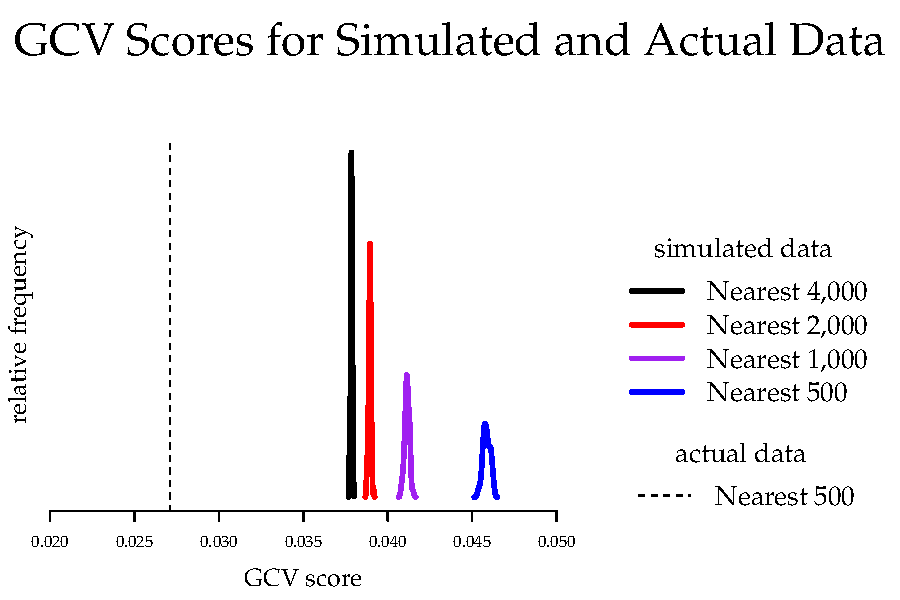
\includegraphics[width=1.1\textwidth]{../graphs/Figure04}}
 \caption{This figure shows the distribution of GCV scores obtained from simulations with spatially randomized data and the GCV score from our data. Each solid curve represents the smoothed density plot of 100 different instances of the simulation. The dashed line suggests that our actual minimum GCV score was not obtained by random chance as no other GCV scores come close.}
 \label{fig:GCVSIM}
\end{figure}

\subsection*{Which Coefficients Vary over Space?}

The previous section presented evidence in support of the claim that there exists significant spatial variation in the hedonic function. However, we have not yet established which variables have spatially varying coefficients. Figures~\ref{fig:AcreBetas}--\ref{fig:NoiseBetas} show the spatial variation in the estimated LWR coefficients for three important variables, lot size, house size, and noise. For comparison, we present the results across four different LWR bandwidths ranging from 500 to 2,000 nearest sales. 

A few patterns are clear. Figure~\ref{fig:AcreBetas} shows that the hedonic coefficient on lot size is largest near the central business district of St.\ Paul. Consistent with standard urban economic theory, to the extent that the hedonic coefficient is correlated with the price of land, our results suggest the price of land is highest near the central business district and declines with distance from the CBD. This tendency is consistent across the different bandwidths, whenever our model ``allowed'' the lot size coefficient to vary over space we saw patterns like these.\footnote{Results for other bandwidths available upon request.} 

The LWR coefficients on house size also seem to exhibit spatial variation in Figure~\ref{fig:HouseBetas}. In the west-central portion of our study area (a collection of notably desirable neighborhoods nestled between the Minneapolis and St.\ Paul CBDs) we see a cluster of large LWR coefficients, while those areas in the southernmost portion of our region (suburban areas) have the smallest coefficients. 

In Figure~\ref{fig:NoiseBetas} we map the estimated LWR noise coefficients from four different bandwidths. In this figure the red areas represent large negative coefficients, while yellow areas are characterized by values closer to zero. The area with the most negative noise coefficients is ringed by some of the coefficients closest to zero (and even greater than zero in some cases) for smaller bandwidths. As the bandwidth increases to 1,000 or 2,000 nearest houses, the variation in noise coefficients decreases substantially. In contrast to the previous two figures, we have largely eliminated the ``hot spots'' that appear in the smaller bandwidths. 


\begin{figure}
 \makebox[\textwidth][c]{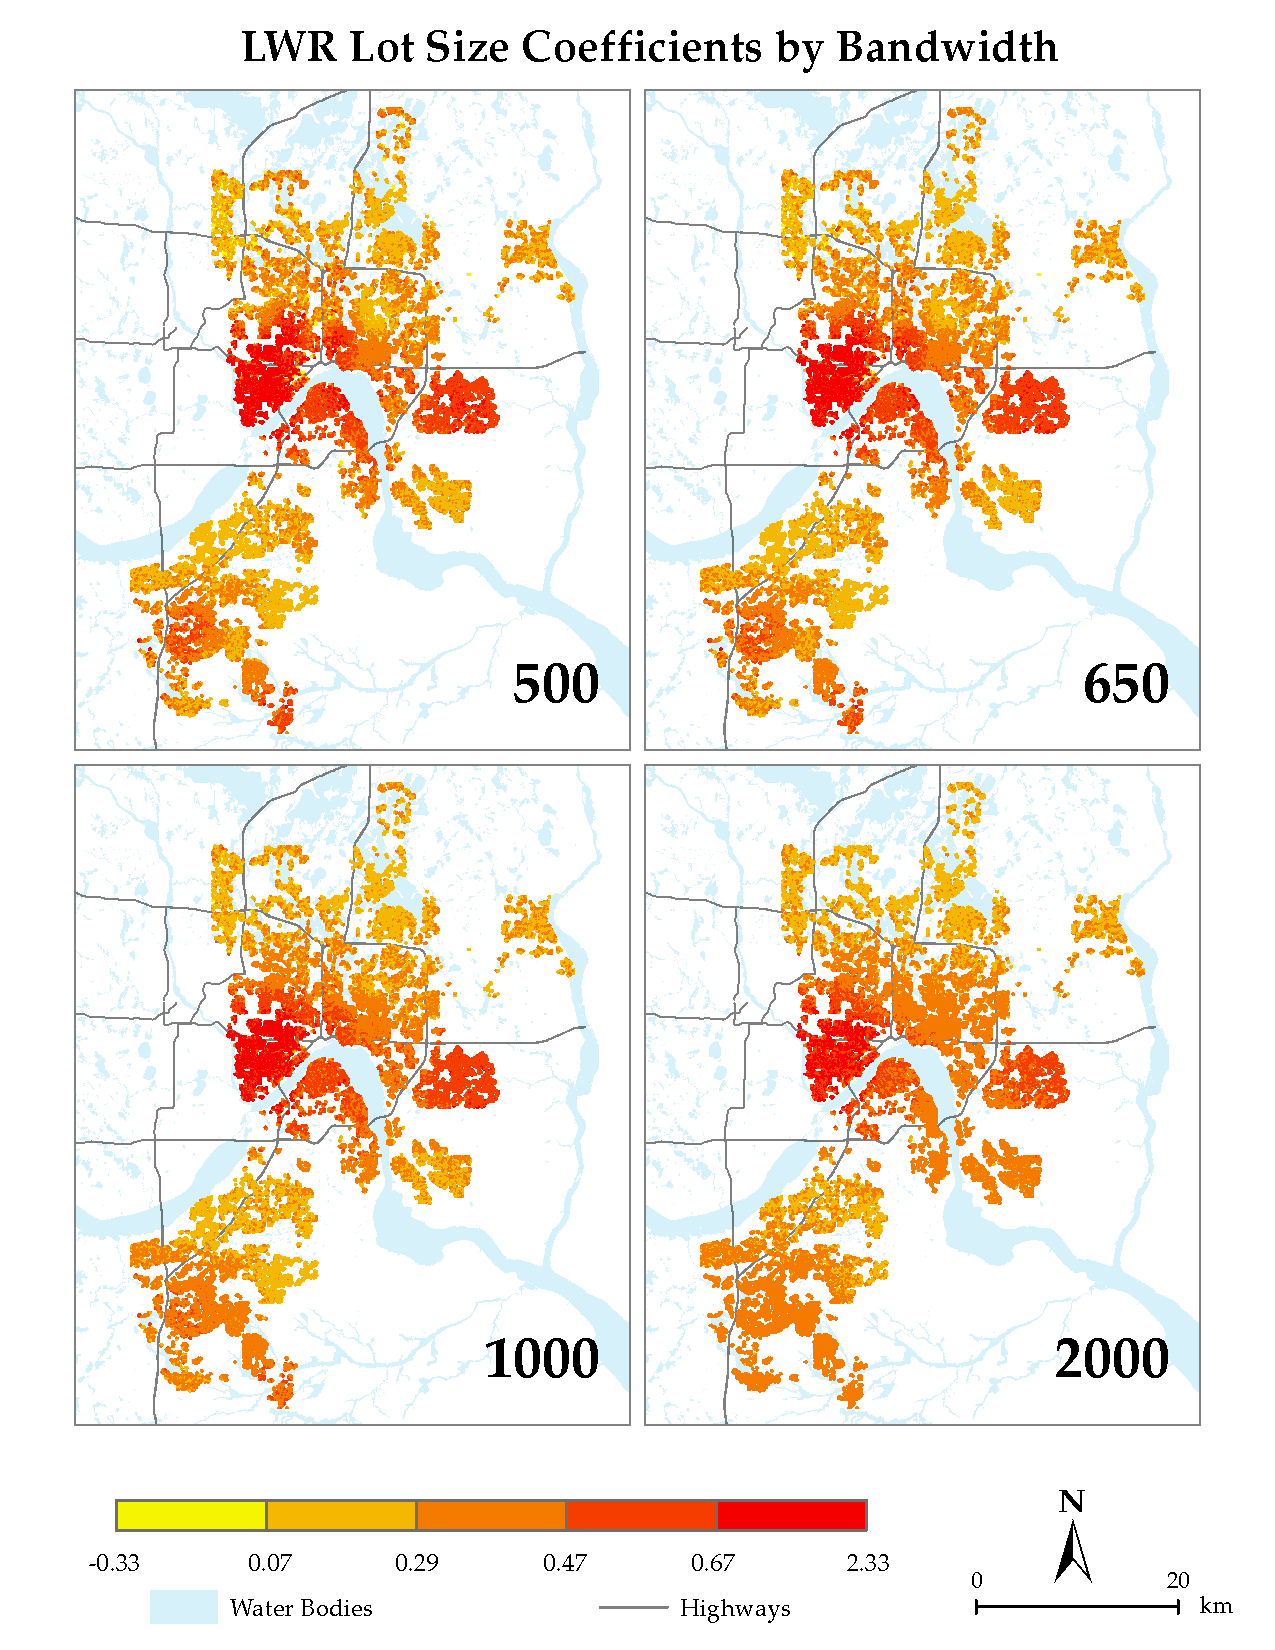
\includegraphics[width=1.1\textwidth]{../graphs/Figure05}}
 \caption{This figure shows an interpolated surface (using Inverse Distance Weighting) for the estimated LWR coefficients (dependent variable = ln(sales price)) for the lot size variable (in acres) obtained across four different bandwidths: 500, 650, 1,000, and 2,000 nearest observations. In all cases there is a clear inverse relationship between the coefficient magnitudes and distance to the central business district.}
 \label{fig:AcreBetas}
\end{figure}

\begin{figure}
 \makebox[\textwidth][c]{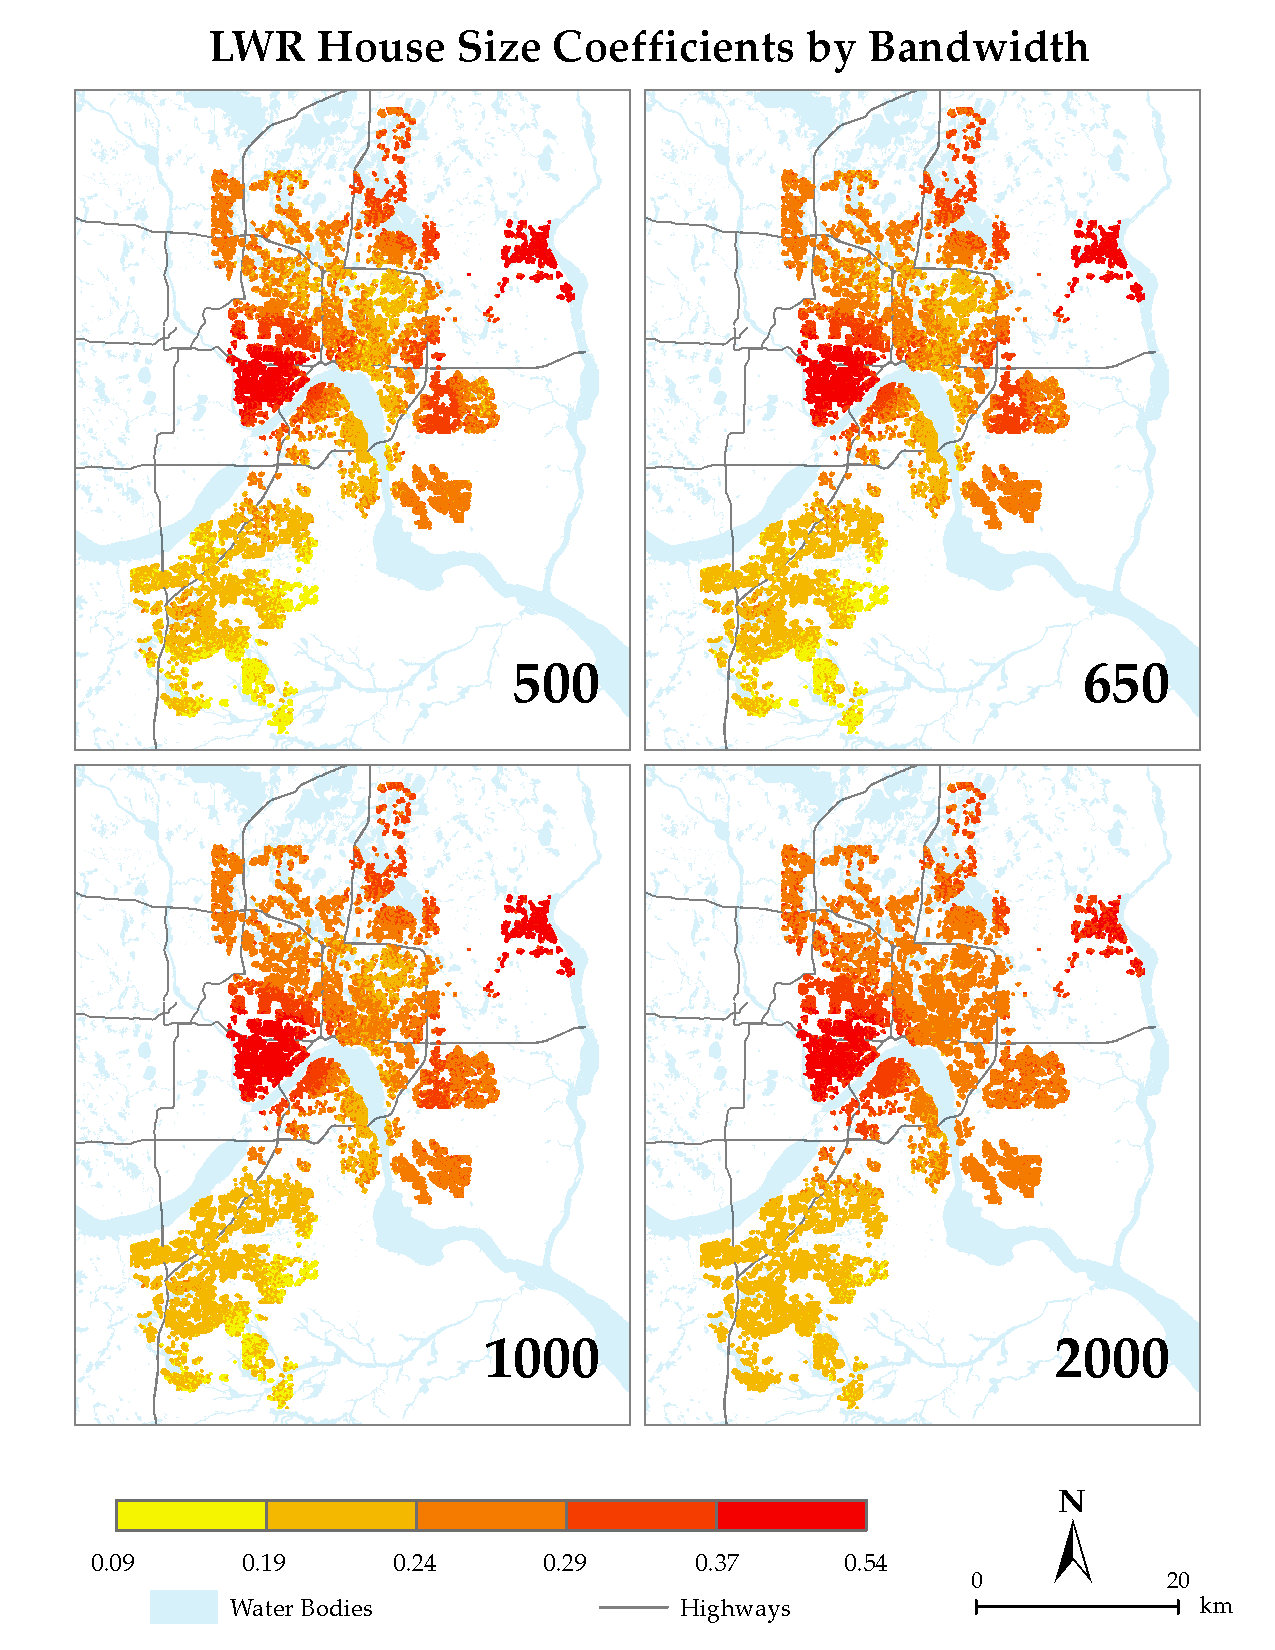
\includegraphics[width=1.1\textwidth]{../graphs/Figure06}}
 \caption{This figure shows an interpolated surface (using Inverse Distance Weighting) for the estimated LWR coefficients (dependent variable = ln(sales price)) for the finished house size variable (in 1,000s of square feet) obtained across four different bandwidths: 500, 650, 1,000, and 2,000 nearest observations. In all cases some of the highest coefficient values are in the west-central portion of our study area and the lowest coefficients tend to be in the far south.}
 \label{fig:HouseBetas}
\end{figure}


\begin{figure}
 \makebox[\textwidth][c]{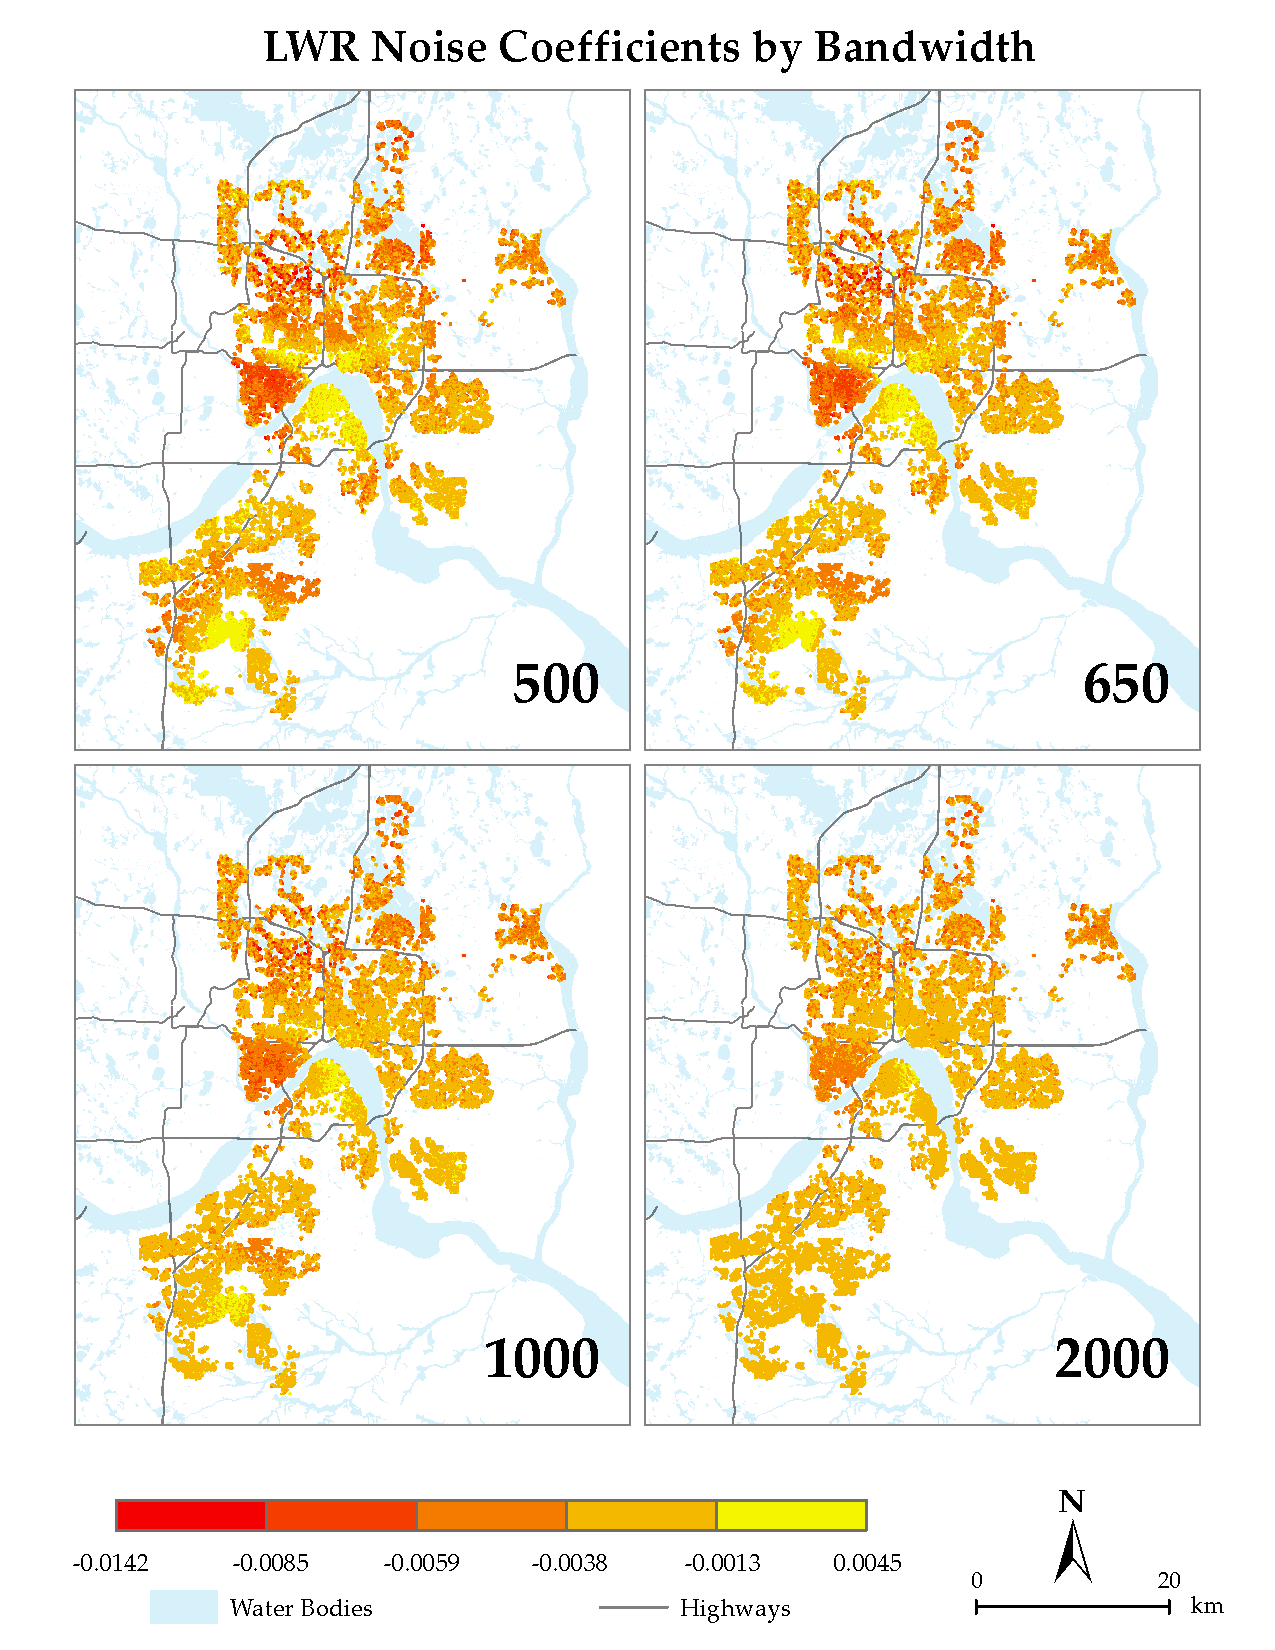
\includegraphics[width=1.1\textwidth]{../graphs/Figure07}}
 \caption{This figure shows an interpolated surface (using Inverse Distance Weighting) for the estimated LWR coefficients (dependent variable = ln(sales price)) for the noise variable (in dB) obtained across four different bandwidths: 500, 650, 1,000, and 2,000 nearest observations. In all cases some of the most negative coefficient values are in the west-central portion of our study area with the smallest in magnitude coefficients tending to be near the central business district.}
 \label{fig:NoiseBetas}
\end{figure}

We conducted a second series of simulation experiments aimed at testing whether the spatial variation exhibited in particular coefficients was significant or due to random chance. The mechanics of the second simulation are very similar to the those described in the previous section. We randomly changed the spatial arrangement of our house sales and re-estimated the LWR model. However, instead of examining the model fit, we compared the \emph{spread} of the regression coefficients (as measured by the standard deviation). If we observed similar levels of dispersion for variable coefficients in the randomly arranged data as in our true data, then we cannot reject the null hypothesis of a stationary relationship. However, significantly \emph{greater} dispersion of regression coefficients with our actual data would provide evidence consistent with the variable having a non-stationary relationship. 

We implemented this experiment 100 times for several different bandwidths and obtained consistent results. For most variables, the standard deviation of the LWR coefficients obtained with our actual data was significantly greater than any standard deviation obtained with the randomized simulated data. We never observed a level of coefficient dispersion anywhere near the actual coefficient standard deviations for variables like house size, lot size, and most others. This can be seen in Figure~\ref{fig:MCsim2} by comparing the dashed lines of a given color to the respective solid colored distributions.\footnote{For brevity's sake we present the results for the 500 and 2,000 bandwidth sizes in Figure~\ref{fig:MCsim2}. Additional results available on request.} However, for variables like noise, owner occupancy and percent of the census block population under age 18, our observed spread in the actual LWR coefficients is similar to the simulated data. In these cases we therefore do not reject the null hypothesis of spatial stationarity. Overall, this simulation suggests that most of our variables seem to exhibit a significant non-stationary relationship with logged sales prices, but noise does not seem to be one of them.

\begin{figure}
 \makebox[\textwidth][c]{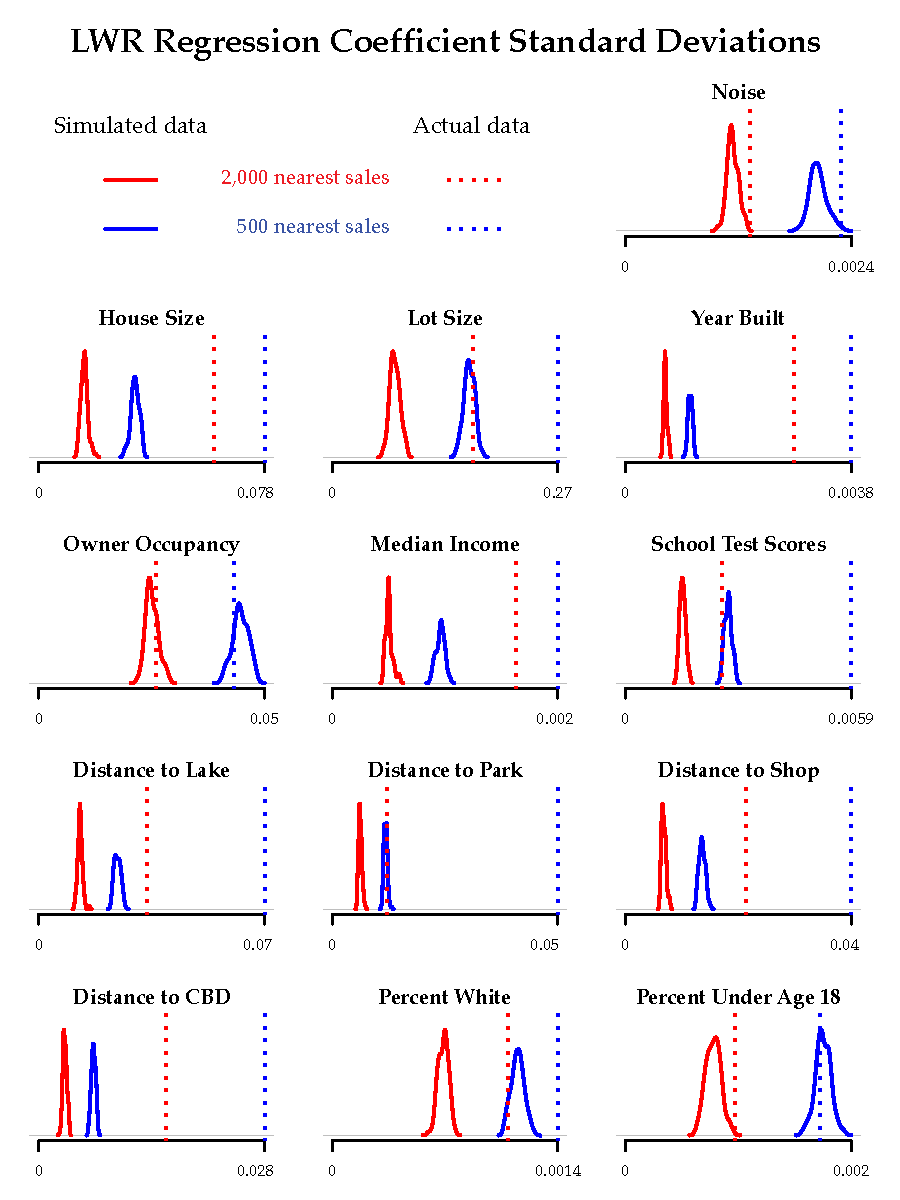
\includegraphics[height=.9\textheight]{../graphs/Figure08}}
 \caption{This figure shows the actual standard deviation in LWR coefficients (dashed line) compared to standard deviations obtained from 100 different instances of spatial randomization (solid lines). Results are presented for two different bandwidths (nearest 500 and 2,000 denoted by color) for each explanatory variable. In all cases the distribution of standard deviations for the smaller bandwidth is larger. In most cases the standard deviation of LWR coefficients for the actual data is substantially higher than any standard deviation obtained with the simulated data, but not for the noise variable.}
 \label{fig:MCsim2}
\end{figure}

\subsection*{Does the Noise Coefficient Change over Time?}

House prices fell dramatically in the United States and in our dataset during and after the Great Recession of 2008-09. We know little about the patterns of change in the hedonic price functions during and after the fall in house prices. Figures~\ref{fig:AcreTime}--\ref{fig:NoiseTime} show the spatial distribution of some our LWR hedonic coefficients for bandwidths of 500 and 2,000 nearest sales for the years 2006--2010.  The estimated LWR coefficients are different over time. In particular, the positive lot size and house size coefficients tend to decrease over time. These results are consistent with standard economic theory, as wealth and income decrease, consumer willingness to pay for normal goods decreases. What is surprising, however, is that the negative noise coefficient estimates also tend to be more negative in later years of our study. Figure~\ref{fig:NoiseTime} shows that the spatial patterns are similar across years (the most negative coefficients tend to be in the same locations across years), but the average noise coefficient tends to be more negative for the later years. 

\begin{sidewaysfigure}
 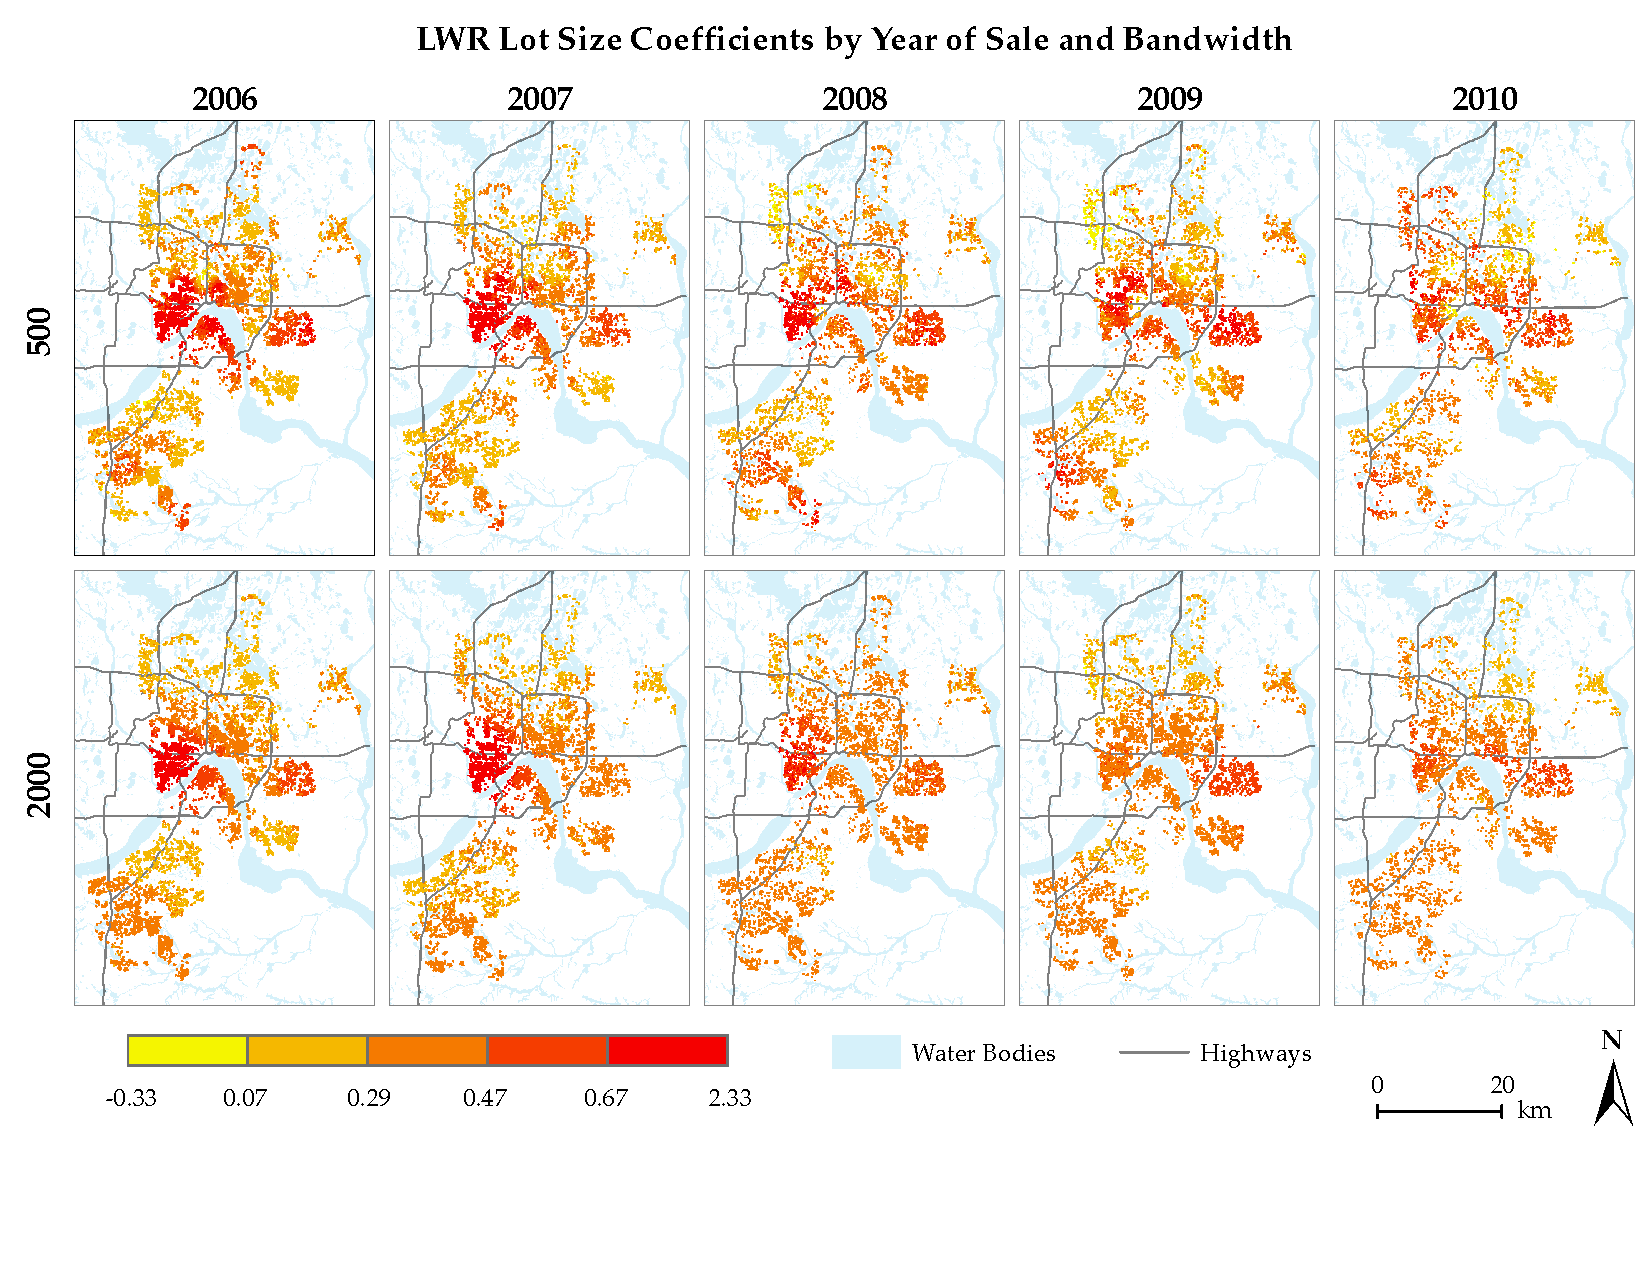
\includegraphics[trim = 0cm 2cm 0cm 0cm, clip = true, width = \textwidth]{../graphs/Figure09}
 \caption{This figure shows the interpolated LWR lot size coefficients across space and time for two bandwidths (nearest 500 and 2,000). Note that the spatial pattern obtained is similar across time periods, but the average value tends to decline over time.}
 \label{fig:AcreTime}
\end{sidewaysfigure}

\begin{sidewaysfigure}
 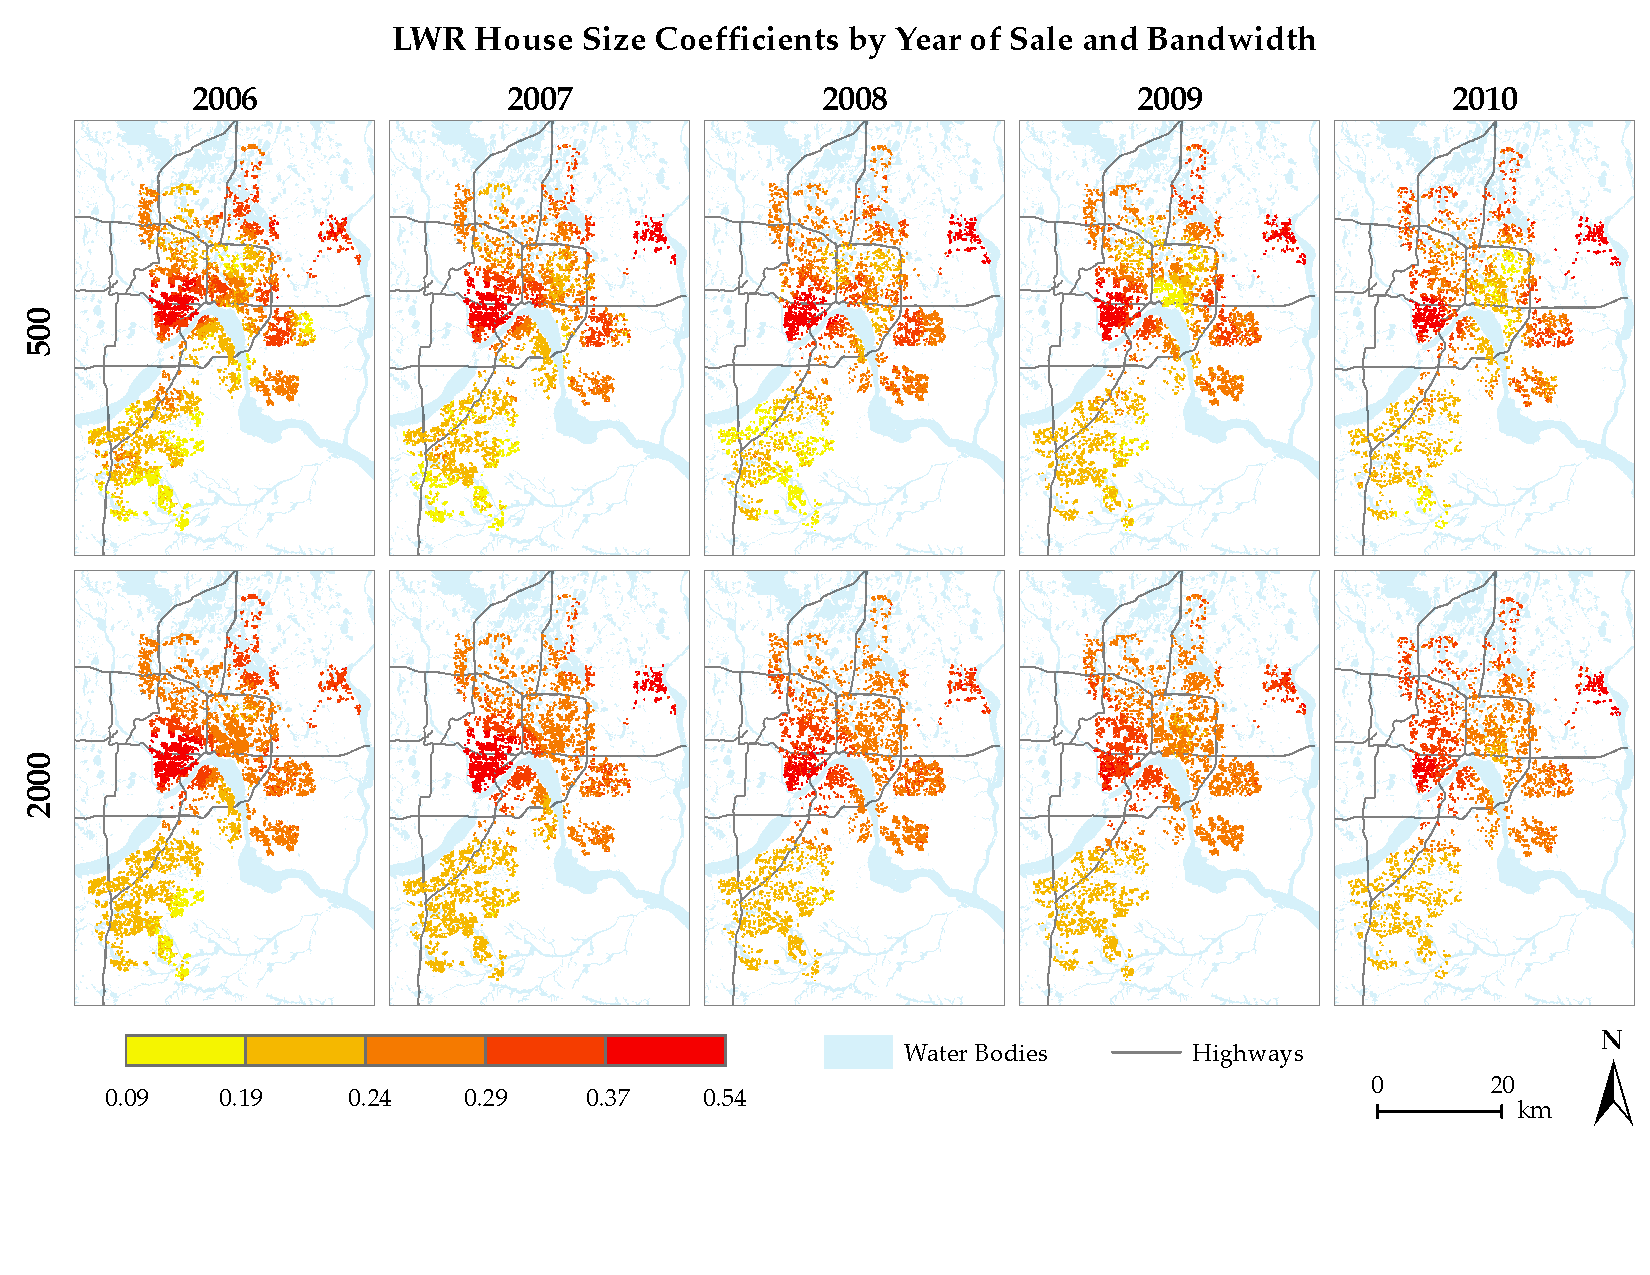
\includegraphics[trim = 0cm 2cm 0cm 0cm, clip = true, width = \textwidth]{../graphs/Figure10}
 \caption{This figure shows the interpolated LWR finished house size coefficients across space and time for two bandwidths (nearest 500 and 2,000). Note that the spatial pattern obtained is similar across time periods, but the average value tends to decline over time.}
 \label{fig:HouseTime}
\end{sidewaysfigure}


\begin{sidewaysfigure}
 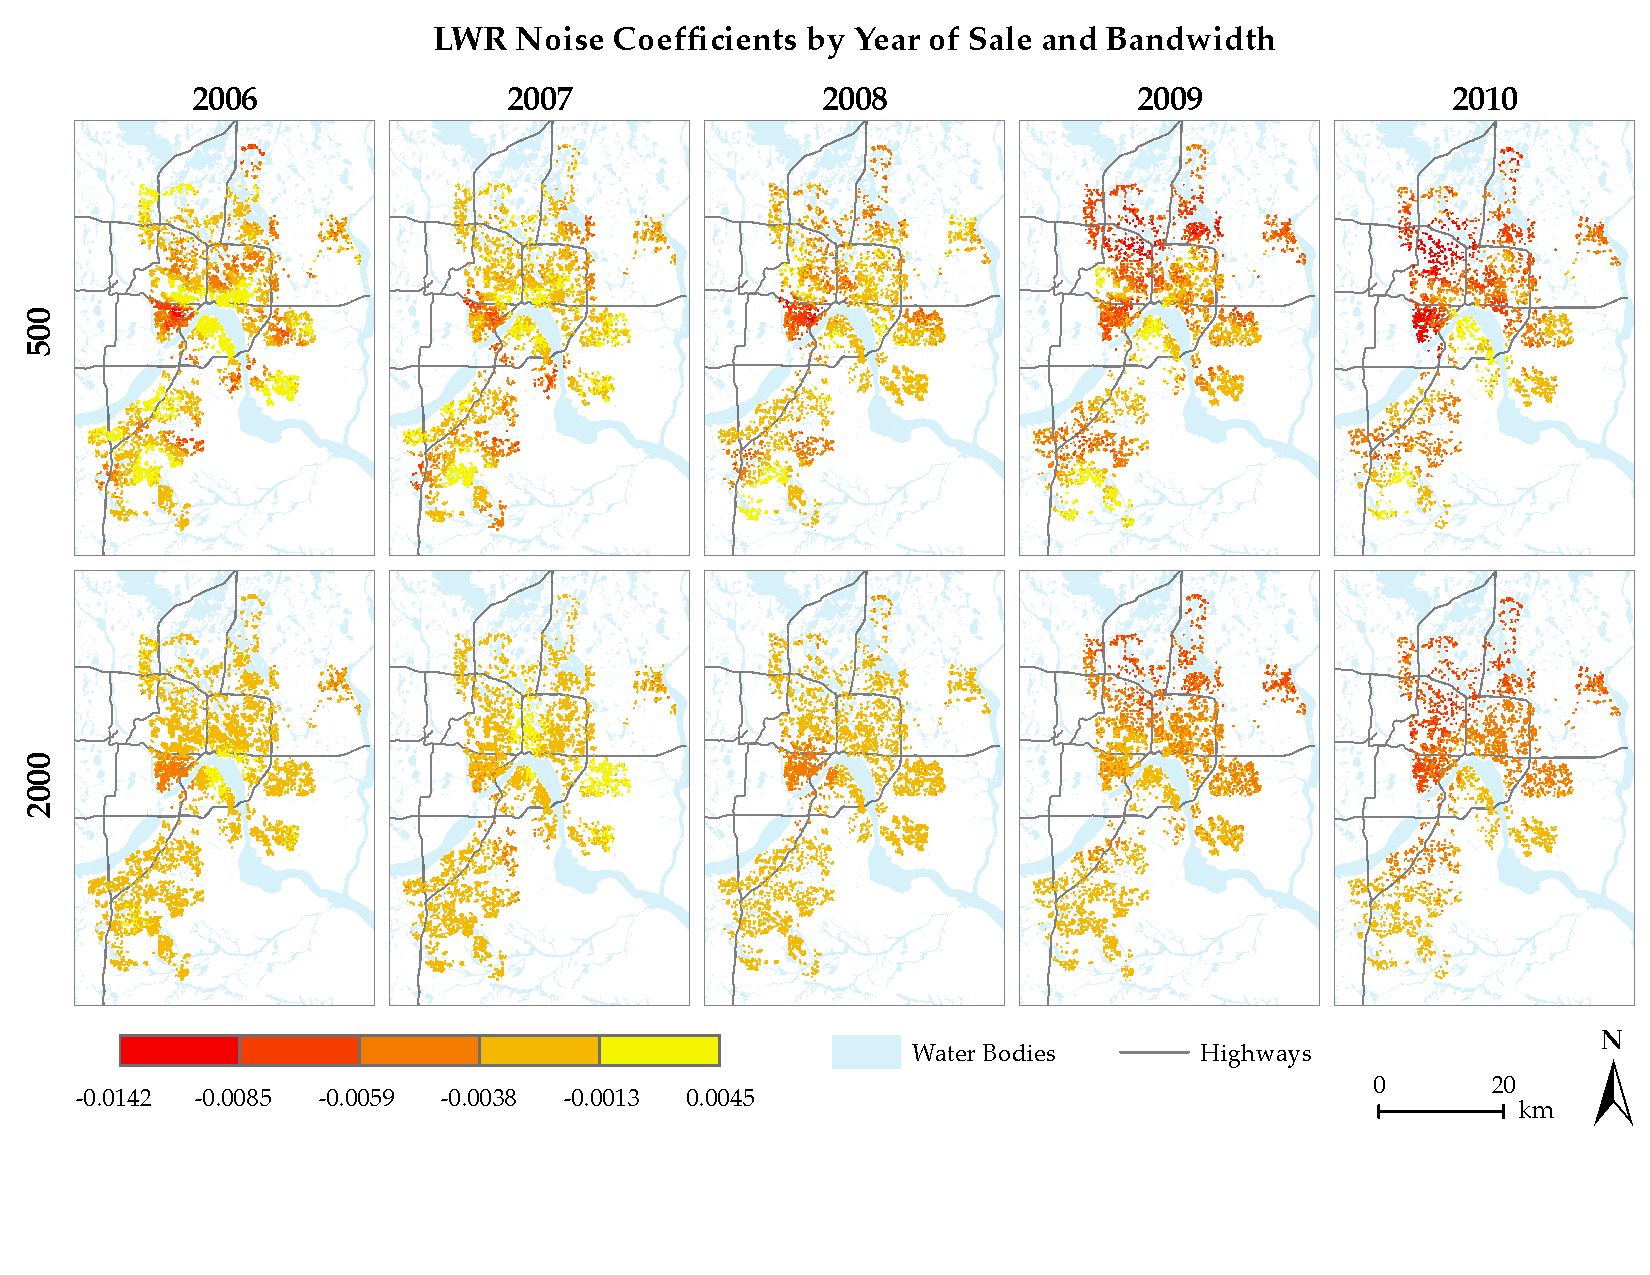
\includegraphics[trim = 0cm 2cm 0cm 0cm, clip = true, width = \textwidth]{../graphs/Figure11}
 \caption{This figure shows the interpolated LWR noise coefficients across space and time for two bandwidths (nearest 500 and 2,000). Note that the spatial pattern obtained is similar across time periods, but the average value tends to decline over time.}
 \label{fig:NoiseTime}
\end{sidewaysfigure}

We also found significant statistical evidence across multiple different formulations and specifications consistent with the estimated noise coefficients being more negative in the later time periods. Tables~\ref{tab:noisebetatime500} and \ref{tab:noisebetatime2000} present the results of regressions using our estimated LWR noise coefficient as the dependent variable and time and spatial characteristics as explanatory variables for LWR bandwidths of 500 and 2,000 nearest sales. Both tables are structured similarly. Column (1) shows a significant negative linear trend in the LWR noise coefficients over time - predicting a LWR noise coefficient of approximately twice the magnitude for the end of our study period as for the beginning. Column (2) includes a significant quadratic term and again predicts noise coefficients much more negative towards the end of our study period compared to the beginning. We repeat the regressions from (1) and (2) in (3) and (4) but this time also included city fixed effects to control for  potential locational differences of house transactions over time. Again, we found very similar results - the noise coefficient is more negative in later time periods. We also limited our analysis to just the city of St.\ Paul and repeated the analysis from (1) and (2) in columns (5) and (6). Again, the noise coefficients were found to be substantially more negative in later time periods. 

% Requires LaTeX packages: dcolumn 
\begin{table}[!htbp] \centering 
  \caption{LWR Noise Coefficient Over Time (bandwidth = 500 nearest sales)} 
    \label{tab:noisebetatime500} 
\scriptsize 
\begin{tabular}{@{\extracolsep{-1pt}}lD{.}{.}{6} D{.}{.}{7} D{.}{.}{7} D{.}{.}{7} D{.}{.}{7} D{.}{.}{7} } 
\\[-1.8ex]\hline 
\hline \\[-1.8ex] 
 & \multicolumn{6}{c}{\textit{Dependent variable: LWR Noise Coefficient (bandwidth = 500 nearest sales)}} \\ 
\cline{2-7} 
\\[-1.8ex] & \multicolumn{1}{c}{(1)} & \multicolumn{1}{c}{(2)} & \multicolumn{1}{c}{(3)} & \multicolumn{1}{c}{(4)} & \multicolumn{1}{c}{(5)} & \multicolumn{1}{c}{(6)}\\ 
\hline \\[-1.8ex] 
Months since Jan 2005 & -0.00005^{***} & 0.00003^{***} & -0.00005^{***} & 0.00003^{***} & -0.0001^{***} & 0.00004^{***} \\ 
  & (0.000001) & (0.000004) & (0.000001) & (0.000004) & (0.000002) & (0.00001) \\ 
  & & & & & & \\ 
 (Months since Jan 2005)$^2$ &  & -0.000001^{***} &  & -0.000001^{***} &  & -0.000001^{***} \\ 
  &  & (0.00000005) &  & (0.00000004) &  & (0.0000001) \\ 
  & & & & & & \\ 
 Constant & -0.0016^{***} & -0.0028^{***} & -0.0021^{***} & -0.0033^{***} & -0.0015^{***} & -0.0032^{***} \\ 
  & (0.00003) & (0.0001) & (0.00003) & (0.0001) & (0.0001) & (0.0002) \\ 
  & & & & & & \\ 
\hline \\[-1.8ex] 
City Fixed Effects & \multicolumn{1}{c}{No} & \multicolumn{1}{c}{No} & \multicolumn{1}{c}{Yes} & \multicolumn{1}{c}{Yes} & \multicolumn{1}{c}{No} & \multicolumn{1}{c}{No} \\ 
\hline \\[-1.8ex] 
Observations & \multicolumn{1}{c}{31,737} & \multicolumn{1}{c}{31,737} & \multicolumn{1}{c}{31,737} & \multicolumn{1}{c}{31,737} & \multicolumn{1}{c}{8,003} & \multicolumn{1}{c}{8,003} \\ 
R$^{2}$ & \multicolumn{1}{c}{0.1273} & \multicolumn{1}{c}{0.1377} & \multicolumn{1}{c}{0.2931} & \multicolumn{1}{c}{0.3028} & \multicolumn{1}{c}{0.1566} & \multicolumn{1}{c}{0.1704} \\ 
\hline 
\hline \\[-1.8ex]  
\end{tabular} 
\end{table} 

% Requires LaTeX packages: dcolumn 
\begin{table}[!htbp] \centering 
  \caption{LWR Noise Coefficient Over Time (bandwidth = 2,000 nearest sales)} 
  \label{tab:noisebetatime2000} 
\scriptsize 
\begin{tabular}{@{\extracolsep{-1pt}}lD{.}{.}{6} D{.}{.}{7} D{.}{.}{7} D{.}{.}{7} D{.}{.}{7} D{.}{.}{7} } 
\\[-1.8ex]\hline 
\hline \\[-1.8ex] 
 & \multicolumn{6}{c}{\textit{Dependent variable: LWR Noise Coefficient (bandwidth = 2,000 nearest sales)}} \\ 
\cline{2-7} 
\\[-1.8ex] & \multicolumn{1}{c}{(1)} & \multicolumn{1}{c}{(2)} & \multicolumn{1}{c}{(3)} & \multicolumn{1}{c}{(4)} & \multicolumn{1}{c}{(5)} & \multicolumn{1}{c}{(6)}\\ 
\hline \\[-1.8ex] 
Months since Jan 2005 & -0.00005^{***} & 0.00003^{***} & -0.00005^{***} & 0.00003^{***} & -0.00005^{***} & 0.0001^{***} \\ 
  & (0.0000003) & (0.000002) & (0.0000003) & (0.000002) & (0.000001) & (0.000004) \\ 
  & & & & & & \\ 
 (Months since Jan 2005)$^2$ &  & -0.000001^{***} &  & -0.000001^{***} &  & -0.000001^{***} \\ 
  &  & (0.00000002) &  & (0.00000002) &  & (0.0000001) \\ 
  & & & & & & \\ 
 Constant & -0.0014^{***} & -0.0026^{***} & -0.0016^{***} & -0.0028^{***} & -0.0016^{***} & -0.0033^{***} \\ 
  & (0.00001) & (0.00003) & (0.00002) & (0.00003) & (0.00003) & (0.0001) \\ 
  & & & & & & \\ 
\hline \\[-1.8ex] 
City Fixed Effects & \multicolumn{1}{c}{No} & \multicolumn{1}{c}{No} & \multicolumn{1}{c}{Yes} & \multicolumn{1}{c}{Yes} & \multicolumn{1}{c}{No} & \multicolumn{1}{c}{No} \\ 
\hline \\[-1.8ex] 
Observations & \multicolumn{1}{c}{31,737} & \multicolumn{1}{c}{31,737} & \multicolumn{1}{c}{31,737} & \multicolumn{1}{c}{31,737} & \multicolumn{1}{c}{8,003} & \multicolumn{1}{c}{8,003} \\ 
R$^{2}$ & \multicolumn{1}{c}{0.3828} & \multicolumn{1}{c}{0.4142} & \multicolumn{1}{c}{0.5128} & \multicolumn{1}{c}{0.5435} & \multicolumn{1}{c}{0.3454} & \multicolumn{1}{c}{0.3988} \\ 
\hline 
\hline \\[-1.8ex] 
\end{tabular} 
\end{table} 

\section{Discussion}\label{Discussion}

Our results have shown a significant negative relationship between house prices and noise, all other things equal. This section describes three important considerations worthy of discussion to help contextualize our results: causation vs.\ correlation, potential temporal problems with our data, and omitted variable bias.

In order to make claims that noise causes a change in house prices, we would ideally observe the same houses over time and randomly ``treat'' some houses with more or less noise to observe the change in price relative to the control houses. Such a study is not feasible with our data and we are therefore limited to a hedonic analysis with observational data. Our conclusions, then, should be interpreted like most other hedonic analysis results and, while we find a strong negative correlation between noise and house prices, we cannot state that noise \emph{causes} lower sales prices. 

Our noise variable is also a model estimate, not a direct measurement of the noise levels encountered by potential house buyers when deciding on their willingness to pay for the property. The model controls for the most important determinants of average noise exposure-- the level of the noise source, the distance and elevation change from the source, the intervening buildings, sound barriers, and foliage, but of course there is undoubtedly error. House purchasers may have visited the property on particularly busy traffic days, or on days with weather conditions more or less conducive to noise propagation across the landscape. Future researchers may seek to collect actual noise exposure data, but this will be a daunting task. 

Our work faces other notable data limitations. While our house sales data were collected over the course of six years, the noise estimates are for the year 2007. To the extent that traffic flows changed with the economic recession, our noise variable could be inaccurate for other years. However, we believe these potential changes are minuscule. Table~VM2 from the US. Department of Transportation Office of Highway Policy Information website\footnote{\url{http://www.fhwa.dot.gov/policyinformation/quickfinddata/qftravel.cfm}} reports that in the year 2007 there were approximately 30 million vehicle miles traveled in the urban areas of the state of MN, while for years 2008, 2009, and 2010 the respective values were 32.5, 32.3, and 32.0 million vehicle miles. Overall, this represents a change of less than 10 percent.  Such small changes in total vehicle miles traveled will not yield significant differences in noise level estimates from our model. Given the computational complexity of re-estimating the landscape noise surface, such work is beyond the scope of this paper, but may be a worthwhile investment for future work seeking to test the robustness of our results.

Our model may suffer from omitted variable bias. For instance, locations exposed to more noise due to their proximity to high traffic areas may also be less safe due to the potential for accidents. Without including a proxy variable for safety, our noise coefficient could be biased - making it appear that home prices are reflecting noise exposure when in fact it could be safety issues. Future research aimed at measuring the impact of noise should continue to seek out and control for other confounding variables. Another identification strategy suggested by an anonymous referee is to collect data on the quality of windows in the house, which would allow for a test of interaction effects between noise and window quality. Unfortunately, such house characteristics were not available for this study.

Our data also omits other common structural characteristics and to the extent that variables like the number of bedrooms, bathrooms, garage size, or construction quality co-vary with other variables in our dataset, our regression coefficients will be biased. We are comforted, however, because we do have some of these important additional variables for a subset of our data. We were able to obtain the number of bedrooms, bathrooms, and garage area for our houses located within Dakota County from the Dakota County Assessor's Office. Our LWR analysis was then repeated on this geographic subset of the data in order to compare our noise coefficients across the different models. We found strikingly similar traffic noise coefficient estimates when these additional structural variables were included and omitted. As shown in Figure~\ref{fig:DAK}, a simple linear regression of the noise coefficient estimates obtained when these additional structural variables were excluded on the estimates obtained when these variables were included yields a line of best fit that is almost indiscernible from the 45 degree line and has $R^2 = 0.96$. 

\begin{figure}
\makebox[\textwidth][c]{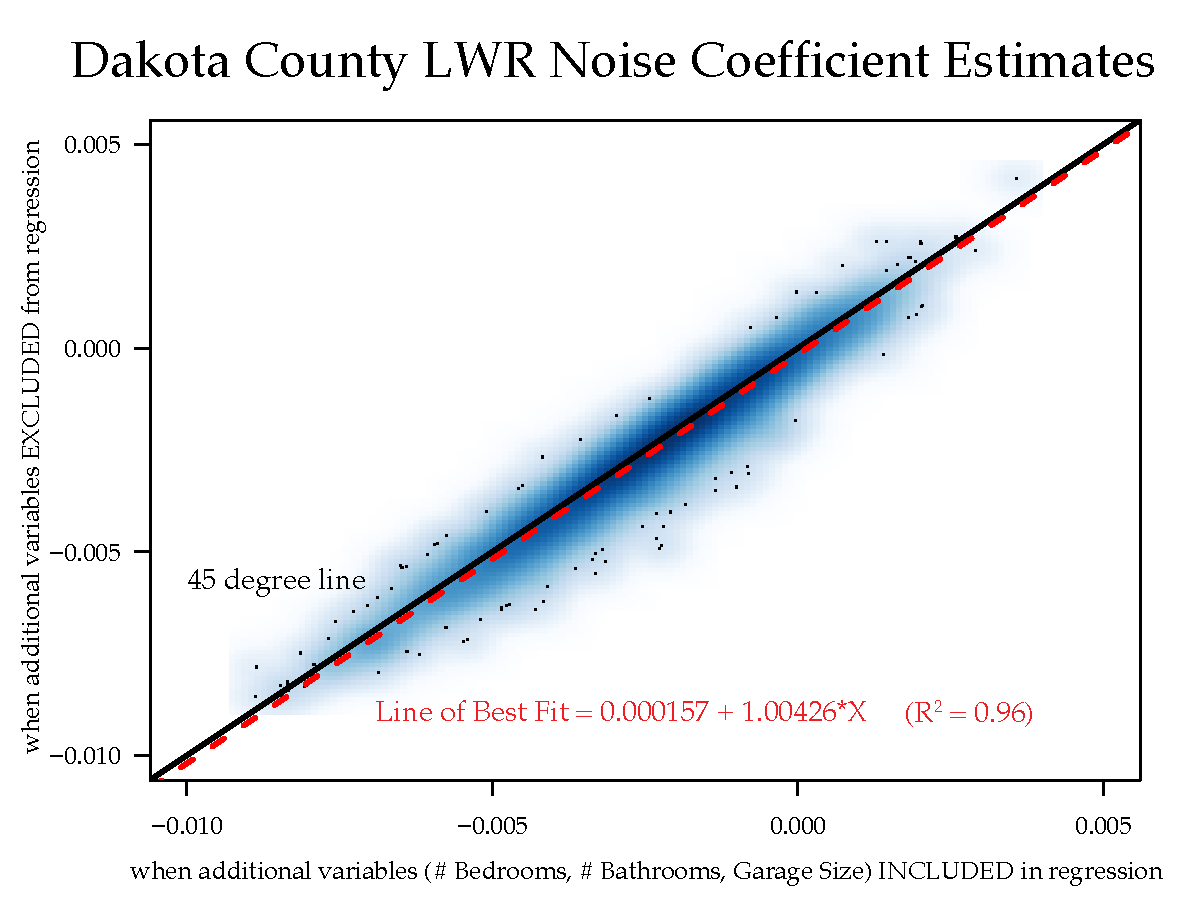
\includegraphics[width = \textwidth]{../graphs/Figure12}}
\caption{This figure shows the similarity between the LWR coefficients we obtained from our model in Dakota County when additional structural variables were excluded vs.\ included in the hedonic regression function. The black line shows the 45 degree line, while the red dashed line shows the estimated line of best fit, which yields a simple $R^2$ of 0.96}\label{fig:DAK}
\end{figure}

\section{Conclusion}
Precise estimates of the impact of traffic noise are important for efficient implementation of noise mitigation projects. The United  States Federal Highway Administration reports that 47 states have constructed noise barriers to reduce noise propagation, spending over a half a billion dollars from 2008-2010 \citepalias{USFHA2012}. \citet{Delucchi1998} used an estimate of 0.85 percent reduction in house prices per additional decibel in their cost-benefit analysis of traffic noise. While their preferred estimate of the total damage cost to the United States in 1991 is \$3 billion, they report a possible range of less than \$100 million to over \$40 billion due in part to uncertainty surrounding the degree of noise propagation over space in the urban built environment and the effect of noise on house prices. Indeed, one of the main conclusions of their work is that more research should be done to better understand the impact of noise on house prices and that better noise data are needed for such work to occur.

We estimated a hedonic price function for single family houses using Locally Weighted Regression techniques in the St.\ Paul, Minnesota, urban area. Specifically, we estimated semi-logarithmic regressions at each house within our dataset using only information contained in ``local'' (both geographically and temporally) house sales. We find strong evidence that the hedonic function in our study area varies over space and time and such flexible models represent significant improvements over conventional parametric models. 

Monte Carlo simulation results suggest that the better goodness-of-fit provided by the local models were not due to chance and that many regression coefficients vary over space within our study area. In over a thousand different trials LWR models with spatially randomized data never fit better than global analysis and we never came close to estimating our observed house sales prices as well as we did with the local analysis on the actual data. Subsequent analysis showed that the standard deviations of most LWR coefficients with the randomized data tended to be much smaller than obtained with our actual data. While our results show very strong evidence that the coefficients on lot size and living space vary over space, the noise coefficient was one of only a few variables to not show evidence of spatial non-stationarity.

We do, however, find significant temporal variation in the noise coefficients-- roughly doubling from a quarter percent per decibel in early 2006 to a half percent per decibel in 2010. Such temporal non-stationarity is consistent with previous work like \citet{Wilhelmsson2000} which found the traffic noise penalty to be stronger in the 1990s near Stockholm, Sweden compared to the 1980s and \citet{Cohen2009} which found the (airport) noise penalty to be larger in the early 2000s compared to the late 1990s in Atlanta, Georgia. However, the significant increase in magnitude is surprising given the severe economic recession and evidence presented by \citet{Cho2011b} that consumers' willingness to pay for environmental amenities (such as proximity to open space and water views) decreased during the recession as compared to the previous economic boom in Nashville, Tennessee.

Future research should be conducted in more housing markets, as the potential to apply the results of analysis in one set of geographical and economic circumstances may be limited. Second, ``mixed'' regression techniques (in which some regression coefficients are constrained to remain constant across the study area while others are allowed to vary) may allow researchers to obtain more precise estimates of the impact of hedonic characteristics by increasing the degrees of freedom in the regression. Lastly, researchers should seek to leverage improvements in spatial hedonic modelling with the advice of  \citet{Carruthers2010} and use the spatial variation in regression coefficients obtained from LWR models to estimate the second-stage hedonic regressions to identify consumer demand curves for these characteristics, thereby further improving our understanding of the value of local amenities.

\newpage
\begin{singlespace}

\input{NoiseHedonicFinalBib.bbl}
\end{singlespace}
\end{document}
